\documentclass[a4paper, 12pt]{ppgeb}

% |--- Títulos, autor, banca ---|----------------------{{{
% Autor:
% Substituta  as informações nos comandos a seguir, até a linha começando
% com \membrobancaexterno.
% Em \title: título na forma principal, como aparecerá em algumas páginas
% Em \tituloficha: título como aparecerá na ficha catalográfica; idêntico
% ao anterior, mas com possíveis quebras manuais de linha (usar \\ quando
% necessário, para ajustar as mudanças de linha na ficha catalográfica).
% Em   \titulocapaA,   \titulocapaB,   \titulocapaC:  título para a capa,
% dividido em no  máximo 3  linhas (coloque uma  linha em  cada  comando,
% dividindo como ficar melhor esteticamente).
% Remova  o  símbolo  de  comentário  (%)  de  \coorientador,  se  houver
% coorientador.
%  Em  \publicacao{011A/2019}:  o  número  final  será   fornecido   pela

\title{Electromyographic\\Signal Processing Using\\Machine Learning and Entropy}
\tituloficha{Electromyographic Signal Processing Using Machine Learning and Entropy\\\phantom{}[Distrito Federal], 2020.} 
\titulocapaA{Electromyographic}
\titulocapaB{Signal Processing Using}
\titulocapaC{Machine Learning and Entropy}
\titulofichadois{Processamento de Sinais Eletromiográficos com o uso de Apredizagem de Máquina e Entropia}
\author{Luiz Barbosa}
\nomeinvertido{Lucas Barbosa, Luiz José}
\orientador{Adson Ferreira da Rocha}
%\coorientador{Nome do Coorientador}
\publicacao{011A/2020}
\data{março de 2020}
\ano{2020}
\areaum{Signal Processing} % Preencher com termos escolhidos para identificar a área
\areadois{Biological Signal Analysis}
\areatres{Information Entropy}
\areaquatro{Machine Learning}
\endereco{contato@luizbarbosa.net}
\cep{CEP 70910-900}

\membrobancainterno{Dr. Cristiano Jacques Miosso}
\membrobancaexterno{Dr. Fabiano Araujo Soares}
%---}}}

% |--- Bibliotecas utilizadas ---|----------------------{{{
\usepackage[margin=1in]{geometry}
\usepackage{setspace}
\usepackage{multirow}
\usepackage{booktabs}
\usepackage{xfrac}
\usepackage{hyperref}
\hypersetup{
colorlinks = true,
linkcolor = black,
anchorcolor = blue,
citecolor = blue,
filecolor = blue,
urlcolor = blue
}
\usepackage{rotating}
\usepackage[margin=0.40in,font=small,labelfont=bf,labelsep=period]{caption}
%---}}}

% |--- Espaçamento, configuração de título de seções ---|----------------------{{{
\onehalfspacing

\makeatletter
\renewcommand{\section}{\@startsection
{section}
{1}
{0mm}
{-\baselineskip}
{0.5\baselineskip}
{\large\bfseries\scshape}}
\makeatother

\makeatletter
\renewcommand{\subsection}{\@startsection
{subsection}
{2}
{0mm}
{-\baselineskip}
{0.5\baselineskip}
{\bf\sffamily}}
\makeatother

\makeatletter
\renewcommand{\subsubsection}{\@startsection
{subsubsection}
{3}
{0mm}
{-\baselineskip}
{0.5\baselineskip}
{\bf\sffamily}}
\makeatother

\setlength{\parindent}{20pt}
\setlength{\parskip}{06pt}
\newcommand{\spaceinitialsname}{0.4mm}
\newcommand{\porcento}{\scalebox{0.5}{~}\scalebox{0.9}{\%}}
\newcommand{\scanner}{\emph{scanner}}
\newcommand{\scanners}{\emph{scanners}}
\newcommand{\cmcubico}{${\textrm{cm}^{\scalebox{0.7}{3} }}$}
\setcounter{secnumdepth}{3}
%\setcounter{tocdepth}{3}
%---}}}

% |--- Comandos especiais ---|----------------------{{{
\newcommand{\cmquad}{${\textrm{cm}^{\scalebox{0.7}{2}} }$}
\newcommand{\mmquad}{${\textrm{mm}^{\scalebox{0.7}{2}} }$}
\newcommand{\gcmquad}{${\textrm{g}}/{\textrm{cm}^{\scalebox{0.7}{2}} }$}
\newcommand{\subsecref}[1]{Seção~\ref{#1}}
\newcommand{\figref}[1]{Figura~\ref{#1}}
\newcommand{\etal}{\emph{et~al.}}
\newcommand{\Jawsonly}{{\emph{Jaws-Only}} }
\newcommand{\jawsonly}{{\emph{jaws-only}} }
\newcommand{\software}{\emph{software}}
\newcommand{\percentagesignscale}{0.8}
\newcommand{\percent}{\scalebox{\percentagesignscale}{~\%}}
\newcommand{\subsubsubsection}[1]{\vspace{16pt}\noindent\textbf{#1}\\[12pt]}
%---}}}

% |--- Diretório(s) com figuras (se desejar, inclua subdiretórios) ---|-------------{{{
\graphicspath{{figuras/}}
%---}}}

% |--- Lista de palavras que não podem ser separadas em sílabas ---|------------------{{{
\hyphenation{development results Commissioning possibility Philadelphia Devic Calculations Calculation Language}
%---}}}

% |--- Texto principal ---|----------------------{{{
\begin{document}

% |- Formato de referências (use apenas uma das 2 linhas seguintes; comente a outra) -|-{{{
\newcommand{\formatobibliografia}{numero}
%\newcommand{\formatobibliografia}{autorano}

\ifthenelse{\equal{\formatobibliografia}{numero}}{
\bibliographystyle{resumoestendido}{plainpt}
\bibliographystyle{mainreferences}{plain}
}
{}

\ifthenelse{\equal{\formatobibliografia}{autorano}}{
\usepackage{apalike}
\bibliographystyle{resumoestendido}{apalikept}
\bibliographystyle{mainreferences}{apalike}
}
{}
%---}}}

\maketitle

% Se desejar uma epígrafe, remova o % do início das próximas linhas (até ==============)
\clearpage
\hspace{1mm}

\vfill

\hspace{1mm}

\begin{center}
\emph{ Suppose that we were asked to arrange the following in two categories — distance, mass, electric force, entropy, beauty, melody. I think there are the strongest grounds for placing entropy alongside beauty and melody, and not with the first three.} \\
Eddington A, The Nature of the Physical World, 1928
\end{center}

\hspace{1mm}

\vfill

\hspace{1mm} 
% ==============

% Se desejar uma dedicatória, remova o % do início das próximas linhas (até ==============)
%\clearpage
%\hspace{1mm}
%
%\vfill
%
%\begin{flushright}
%\begin{itshape}
%Texto da dedicatória.
%\end{itshape}
%\end{flushright}
% ==============

% Se desejar incluir agradecimentos, remova o % do início das próximas linhas (até ==============)
\clearpage
\noindent{\bfseries{\maiusc{\large Agradecimentos}} }

\vspace{24pt} Agradeço aos meus colegas de laboratório e trabalho pelas ajudas, conversas e insights. Agradeço também ao meu orientador, Adson, por sua ajuda, conselhos e guias. Principalmente agradeço ao meu co-orientador Alberto, que sem ele não teria conseguido concluir esse projeto.

\noindent 
\clearpage
% ==============

\newgeometry{bottom=0.8in, top=0.9in, left=0.9in, right=0.9in}

\noindent{\bfseries{\maiusc{\large Resumo Estendido}} }
\acresetall % Manter essa linha!
\vspace{12pt}

O sinal eletromiográfico é utilizado em diversas áreas da Medicina e da Biologia, em especial na área de reabilitação muscular. Uma aplicação importante é no no controle de próteses robóticas. Atualmente, diversas próteses comerciais de mão utilizam uma malha de controle sequencial, o que torna o movimento da prótese pouco fluido e dependente de sensores externos para execução de movimentos. O presente plano de trabalho propõe o desenvolvimento deum estudo de métodos para o uso sinal da eletromiografia de superfície (sEMG) para o controle em tempo real de uma prótese de mão. O objetivo é utilizar métodos de extração de características e classificação de padrões em sinais eletromiográficos, assim como o treinamento adaptativo para o reconhecimento de movimentos da mão com vários graus de liberdade, aumentando assim o conforto do usuário e dando naturalidade ao movimento. Por meio desses métodos, foi obtido uma melhoria significativa no processo de reconhecimento de padrões. As propostas e métodos de classificadores foram desenvolvidas e testadas com o uso das bases de dados disponíveis na plataforma \textit{Open Source} BioPatRec~\cite{resumoestendido}{Ortiz-Catalan2013}, a linguagem utilizada para os algoritmo foi o python, com o auxilio das bibliotecas Scikit-learn~\cite{resumoestendido}{scikit-learn}, ScyPy~\cite{resumoestendido}{2019arXiv190710121V} e Tensorflow~\cite{resumoestendido}{Abadi2016}. Diversos indicadores estatísticos, são aplicados para avaliar o reconhecimento de padrões, \textit{off-line} e \textit{on-line}.

\vspace{14pt}

\noindent\textbf{Palavras-chave: sinal eletromiográfico de superfície, prótese de mão, reconhecimento de padrões, redes neurais, entropia.}

\secaoresumo{Introdução}
Segundo o IBGE~\cite{resumoestendido}{IBGE2010}, no Brasil, 13,2 milhões de pessoas se declararam portadoras de algum tipo de deficiência motora, sendo que 470 mil foram vítimas de amputações. Uma amputação de mão é uma das lesões mais prejudiciais e pode afetar dramaticamente as capacidades de uma pessoa. Estima-se ainda, segundo o IBGE, que a incidência média anual de amputações seja de 13,9 por 100 mil habitantes. Além disso, segundo dados do Ministério da Saúde~\cite{resumoestendido}{MinisteriodaSaude2015}, o total de nascidos vivos no Brasil no ano de 2015 foi de 3.017.668 e, sabe-se que, de 1 a 2\% deles sofrem de alguma anomalia congênita e destes, aproximadamente 10\% possuem deformidades dos membros superiores~\cite{resumoestendido}{MinisteriodaSaude2015,SH2003, SH2004}.

Houve grandes avanços nas interfaces homem-máquina, na qual os sinais biomédicos, como os sinais mio-elétricos, desempenham um papel fundamental. O controle utilizando o sinal mio-elétrico é uma técnica avançada, subdividida em detecção, processamento, classificação e aplicação de sinais EMG para controlar robôs ou dispositivos de reabilitação humanas. Os sinais mio-elétricos são muito ricos em informações, a partir das quais a intenção de movimento do usuário em forma de contração muscular pode ser detectada, usando eletrodos de superfície. O sinal da eletromiografia de superfície é detectado de forma não invasiva a partir da superfície da pele e pode ser adaptado para força proporcional ou controle de velocidade em um esquema de controle.

Os sinais de eletromiografia possuem uma propriedade não estacionária, que dificulta a aplicação de reconhecimento de padrões mio-elétricos para o controle de próteses. Na literatura, o reconhecimento de padrões EMG é separado em duas etapas separadas, uma de treinamento e outra de teste. Porém nessa análise não são consideradas as mudanças entre o treinamento e os dados de teste induzidos por mudança de eletrodo, fadiga muscular, mudanças de impedância e fatores psicológicos, que muitas vezes resulta em queda do desempenho~\cite{resumoestendido}{Roche2014}. Para solucionar esse problema, vários estudos sobre treinamento adaptativo vem sendo feitos~\cite{resumoestendido}{Amsuss2014,Diehl,Jain2012,Roche2014,Tommasi2013,Yang2011}, a fim de manter a taxa de certeza da análise do sinal sEMG.

Como os dados do sinal EMG são adquiridos em um curto período de duração, os parâmetros coletados contêm informações limitadas, que não representam todo o período de utilização da prótese. Ampliar o tempo de coleta de dados se torna impraticável, pois adicionaria uma carga muito grande ao usuário. Os sistemas de próteses que utilizam controle de reconhecimento de padrões mio-elétricos não são comercializados por possuírem desempenho insatisfatório~\cite{resumoestendido}{Peerdeman2011}, justamente por causa das variações dos dados de teste em relação aos do treinamento. Portanto, torna-se necessário desenvolver um sistema de aprendizado que consiga se adaptar e contabilize as mudanças do sinal do EMG. Mais especificamente, para que a prótese se torne o mais natural possível, é necessário que se faça uma reconfiguração gradual do classificador de forma online, levando em consideração as mudanças em tempo real do sinal EMG.

As principais empresas que comercializam próteses, no mundo, são a Touch Bionics, Otto Bock, Steeper e Vicent GmbH. Todas as próteses fabricadas por elas possuem um controle sequencial, sendo que algumas delas possuem sensores para auxiliar a movimentação da prótese ou movimentos já predefinidos~\cite{resumoestendido}{Geethanjali2016}. Isso demonstra que o caminho para o controle natural ainda é longo, o que limita a usabilidade da prótese a apenas um membro de apoio. O controle simultâneo visa dar naturalidade ao movimento da prótese, diminuindo o seu desconforto que pode levar ao abandono da mão biônica~\cite{resumoestendido}{Brook1985,McFarland2010}.

\secaoresumo{Importância da Informação no Sinal EMG}
A busca e o processamento de informações são um processo cognitivo complexo que exige a identificação extração e organização da informação relevante. Porém, com a evolução da computação em nuvem, técnicas de classificação baseadas em Deep Learning cresceram muito, uma vez que elas veem performando melhor do que técnicas convencionais de Machine Learning. Esse aumento no uso de técnicas de Deep Learning faz com que muitas vezes não seja necessário entender o problema ou delimitar suas bordas.

Essa abordagem gera um problema, como não houve um aprendizado do processo, o resultado fica dependendo da rede neural e ao que ela foi treinada a fazer. Outro problema é que o conhecimento ganho pode ser usado para outras aplicações.

Em 1948, Claude Shannon publicou um artigo chamado Teoria Matemática da Comunicação~\cite{resumoestendido}{C.E.Shannonvol.27pp.JulyOctober1948}. Neste artigo, Shannon descreve como a informação pode ser comunicada por diferentes elementos de um sistema. Shannon mostra como sinais e ruídos se relacionam e como a habilidade de separa-los para extrair informação dos dados é crucial para o processo de comunicação.

A informação é normalmente medida em bits e, um bit de informação permite a escolha de duas alternativas igualmente prováveis. Como exemplo, temos o lançamento de uma moeda, ao se revelar o resultado, é gerado um bit de informação.

A teoria da informação tem os seus próprios conjuntos de termos. Uma mensagem é o uma sequencia ordenada de símbolos. Uma mensagem composta por símbolos \(\textbf{s} = (s_1, ..., s_n) \) é codificada por uma função \( \textbf{c }= f(\textbf{s})\) em uma sequencia de códigos \(\textbf{c} = (c_1, ..., c_m)\), aonde o número de símbolos ou códigos não são necessariamente iguais. Esses códigos são transmitidos por um canal de comunicação para produzir saídas \(\textbf{y} = (y_1, ..., y_k)\) que são decodificadas para reconstruir a mensagem \(\textbf{s}\).

\secaoresumo{Introdução à Entropia}

Ainda segundo Shannon~\cite{resumoestendido}{shannon1949mathematical}, Para que as definições matemáticas da informação sejam uteis, elas precisam obedecer as seguintes propriedades:
\begin{enumerate}
\item \textbf{Continuidade:} O total de informação associado à um resultado aumenta ou decrementa  continuamente, de acordo com a mudança da probabilidade do resultado.
\item \textbf{Simetria:} O total de informação associado com uma sequencia de resultados não depende da ordem em que os resultados acontecem.
\item \textbf{Valor máximo:} O total de informação com um conjunto de resultados não pode aumentar se esses resultados são igualmente prováveis.
\item \textbf{Adição:} A informação associada com um conjunto de resultados é obtida pela adição das informações dos resultados individuais.
\end{enumerate}

\textbf{Surpresa e Entropia}

Quanto mais improvável é um resultado, mais surpresa é tida com a sua observação. Então o total de surpresa associado a um resultado aumenta, caso a probabilidade do resultado diminua. Então, para satisfazer a condição de aditividade, Shannon utilizou o logaritmo de \(1/p(x)\).  Isto é conhecido como informação de Shannon de \(x\), ou seja a informação de Shannon é uma medida da surpresa. A surpresa média de uma variável \(X\), com uma distribuição \(p(X)\) é chamada entropia de \(p(X)\) e, é representada por \(H(X)\).

\begin{equation} \label{eq:re}
H(X) \approx \frac{1}{n} \sum_{i=1}^{n} log(\frac{1}{p(x_i)})
\end{equation}

Basicamente, entropia é a medida de incerteza. Quando a incerteza é reduzida, informação é ganha. Portanto, se a incerteza de uma variável \(X\) é resumida por sua entropia \(H(X)\), se o valor de \(X\) for revelado, o total de informação ganha é, na média, exatamente igual a entropia.

Caso hajam valores consecutivos e relacionados, então eles não fornecem informação independente. Nesse caso a sequencia possui menos entropia do que o somatório das entropias individuais calculados com a \autoref{eq:re}. Assim, o teorema de Shannon não se aplica apenas a sequencias de elementos independentes, mas também para sequencias estruturadas que possuem dependências entre os seus elementos.

\secaoresumo{Entropia e o sinal sEMG}

O sinal sEMG, assim como todos os sinais naturais, é um sinal diluído, isto é, um sinal que possui muitos dados e pouca informação. Ademais ele é um sinal em que cada sequencia de amostragem possui um alto grau dependência entre seus valores.

\textbf{Processamento em tempo real}

Como uma boa experiência em prótese precisa de respostas rápidas, o processamento em tempo real é essencial. Radhika Menon, et al~\cite{resumoestendido}{RadhikaMenonStudentMemberIEEEGaetanoDiCaterinaHebaLakanyMemberIEEELykourgosPetropoulakisBernardA.ConwayJohnJ.SoraghanSeniorMember} mostra o impacto do tamanho da janela temporal no erro da classificação do sinal sEMG. Segundo esse estudo com janelas muito pequenas, em média menores do que 200 ms o erro da classificação aumenta, uma vez que o total de informação na janela diminui. Isso dificulta muito o processamento em tempo real que precisa de janelas, em 2011 Peerdeman~\cite{resumoestendido}{Peerdeman2011} constatou que a janela de processamento precisa ser menor do que 300 ms ou o atraso se torna inaceitável para o usuário. Instintivamente nota-se a necessidade da diminuição da janela de tempo de processamento para o aumento do conforto do usuário.

Uma das dificuldades na classificação do sinal geradas pelo tamanho reduzido da janela temporal foi identificar exatamente onde o movimento começou. Isso ocorre devido às características estocásticas do sinal, quando as unidades motoras começam a ser recrutadas, o sinal de repouso e movimento é confundido.

Para diferenciar esses dois estados, foi utilizado um autoencoder variacional. Devido a suas características intrínsecas, ele é especializado em separar classes (movimento e repouso) em sua camada latente. Após essa separação, uma percepção simples, foi o suficiente para classificar esses estados.

\textbf{Extraindo informação do sinal}

Para extrairmos informação da eletromiografia de superfície, foi utilizada uma técnica conhecida como extração de características. O sinal foi dividido em janelas de 50 ms, aonde o sinal sEMG é analisados e as características baseadas em frequência são extraídas, seguindo os principais recursos selecionados e finalmente, a rede neural classifica o movimento.

As características extraídas são:
\begin{enumerate}
\item SpectralMoment;
\item Sample Entropy;
\item KhushabaSet;
\item Wave Lenght (frequency);
\item Mean Frequency;
\item Meadian Frequency.
\end{enumerate}

\secaoresumo{Metodologia}

A utilização de técnicas de reconhecimento de padrões é de grande importância para o controle de próteses mio-elétricas, trazendo uma melhora nos graus de liberdade e movimentação das mesmas além da capacidade de seu controle sequencial~\cite{resumoestendido}{Englehart2003}. Tal controle consiste tipicamente na extração de características do sinal e na classificação destas características de dados segmentados no processamento de sinal para comando de um atuador. A qualidade da movimentação dessas próteses é proporcional aos processos de extração das características do sinal mio-elétrico e da classificação dos padrões.

Conforme já mencionado, a maioria dos sistemas de controle empregados em mãos prostéticas é o controle sequencial, mas, recentemente, muitas pesquisas estão sendo conduzidas para empregar o controle simultâneo~\cite{resumoestendido}{Bennett2017,Dosen2015,RadhikaMenonStudentMemberIEEEGaetanoDiCaterinaHebaLakanyMemberIEEELykourgosPetropoulakisBernardA.ConwayJohnJ.SoraghanSeniorMember,Young2013}. Uma das principais vantagens do controle simultâneo da prótese é aproximar a movimentação da prótese ao movimento fisiológico natural, porem isso leva a um aumento das características necessárias para se classificar o sinal, além da interferência do sinal de músculos adjacentes nos eletrodos de captura do sEMG.

\textbf{Clusterização, máquina de estados e a classificação do movimento}

O idioma inglês possui uma dívida a Shakespeare. Ele inventou mais de 1700 de palavras, transformando substantivos em verbos, ou verbos em adjetivos, ou conectando palavras nunca antes usadas em conjunto, ou ainda adicionando prefixos e sufixos e criando palavras totalmente originais. Assim como o inglês consiste de sequencias de letras não independentes que podem ser eficientemente codificadas como blocos independentes de sub-sequencias, assim também pode ser feito como a maioria dos sinais naturais, como música, imagem, DNA, ou o EMG.

Para a classificação do sinal EMG foi realizado um janelamento no sinal, cada janela com 10ms. Após este janelamento foi realizado as seguintes etapas:
 
\begin{enumerate}
    \item Seleção de características: nesta etapa diversos características, tanto no domínio da frequência quanto no domínio do tempo serão extraídas;
    \item Redução de dimensionalidade: nesta etapa diversos algoritimos de redução de dimensionalidade foram avaliados para a criação de clusters de sinais de movimentos parecidos. Foram avaliados:  NCA (Neighborhood Component Analysis), PCA (Principal Component Analysis), LDA (Linear Discriminant Analysis), Variational Autoencoders;
    \item Clusterização do sinal: após avaliação de diversos algorítimos de de clusterização, os movimentos foram agrupados em grupos de acordo com a similaridade das características extraídas;
    \item Comparação com os possíveis movimentos: após o cluster ser criado, os movimentos são comparados com os possíveis movimentos para determinada posição. Esses movimentos foram extraídos através de um processo chamado de Árvore de Decisão ou Máquina de Estados~\cite{resumoestendido}{Villarejo2014};
    \item Classificação do sinal: com a redução das possíveis classes de movimento em intercessão com os clusters criados, diversos classificadores são criados com subconjuntos das classes totais de movimentos.
\end{enumerate}

Cada janela de tempo retorna uma resposta para os possíveis movimentos, o cluster o qual o movimento pertence e a possível classificação. Essas respostas podem ser consideradas letras em uma sentença. Cada janela retorna uma sequencia dependente da sequencia anterior e aonde acada uma das janelas diminui a entropia do sinal como um todo.

\secaoresumo{Resultados e Discussões}
Desde que as próteses mio-elétricas foram desenvolvidas, o número de usuários que a rejeitam permaneceu constante~\cite{resumoestendido}{Brook1985,McFarland201}, O que mostra que não houve avanço significativo na área. A redução da janela de tempo para a classificação do sinal EMG permitirá que o controle da prótese seja realizado de forma mais fluida pelo usuário, aumentando seu conforto ao utilizá-la. 

Outro fator muito importante gerado pela diminuição da A janela de tempo diminui a complexidade da avaliação, o que resulta em economia de energia durante o processo de classificação, o que, por sua vez, aumentaria o tempo de uso da prótese, reduzindo o tempo de recargas que o usuário precisaria fazer. 

Além disso, o processamento desenvolvido neste estudo pode ser usado para a classificação de outros sinais naturais que, à medida que são diluídos (muitos dados para pouca informação), são difíceis de classificar.

\secaoresumo{Conclusão}

Ao fornecer informações a priori para classificação de sinais interativamente, o número de classes possíveis para classificação de sinais diminui bastante. Criar etapas de validação menos complexas também aumentou a precisão, permitindo a redução do tamanho da janela. 

As técnicas apresentadas aqui apenas arranham a superfície das aplicações em que a entropia de formações pode e deve ser usada. A ideia principal é que uma sequencia de redes simples cuja descrição precise de um pequeno número de bits tenha maior probabilidade de generalizar corretamente do que uma rede mais complexa, porque presumivelmente extraiu a essência dos dados e removeu a redundância. Portanto, fornecer ferramentas que simplifiquem ou forneçam informações de dados é muito importante.

Infelizmente, a coleta de dados do sinal EMG pode ser estressante para o paciente. Portanto, é muito difícil obter grandes bancos de dados de sinais biológicos. Por esse motivo, este estudo foi realizado usando apenas um banco de dados, fornecido junto com a plataforma BioPatRec. Além disso, o banco de dados utilizado possui poucas repetições de movimento, o que dificulta o treinamento com algoritmos de aprendizado de máquina. 

No total, essa base possui apenas 17 pacientes e 3 repetições de cada movimento, o que impossibilitou o uso de algumas técnicas de treinamento. Com um banco de dados suficientemente grande e, uma vez criado um classificador redundante, como no caso do estudo, os diversos As etapas da classificação podem ser usadas como um código e, com uma rede neural maior, e os valores das janelas de classificação podem ser previstos usando técnicas como LSTM. A relação de dependências entre as janelas de tempo também pode ser estudada para se obter um classificador melhor projetado.

{\let\clearpage\relax
\bibliography{resumoestendido}{referencias}{\scalebox{0.7}{Lista de Refer\^{e}ncias}}
}
\acresetall % Manter essa linha!
\clearpage
\restoregeometry
% \chapter{Abstract}
\noindent{\bfseries{\maiusc{\large Abstract}} }
\acresetall % Manter essa linha!
\vspace{24pt}

The electromyographic signal is used in several areas of medicine and biology, especially in the muscle rehabilitation area. Another important application is in the control of robotic prostheses. Currently, several commercial hand prostheses use a sequential control loop, which makes the movement of the prosthesis less fluid and dependent on external sensors to perform movements. The present work plan proposes the development of a study of methods for the use of surface electromyography signal (sEMG) for real time control of a hand prosthesis. The objective is to use methods of feature extraction and pattern classification in electromyographic signals, as well as adaptive training for the recognition of hand movements with varying degrees of freedom, thereby increasing user comfort and giving the movement a natural feel. Through these methods, a significant improvement in the pattern recognition process was obtained. The proposals and methods of classifiers were developed and tested using the databases available on the Open Source BioPatRec ~\cite{mainreferences}{Ortiz-Catalan2013} platform, the language used for the algorithms was python, with help from the Scikit-learn ~\cite{mainreferences}{scikit-learn}, ScyPy ~\cite{mainreferences}{2019arXiv190710121V} and Tensorflow ~\cite{mainreferences}{Abadi2016} libraries. Several statistical indicators are applied to assess pattern recognition, offline and online.

\vspace{14pt}

\noindent\textbf{Keywords: surface electromyographic signal, hand prosthesis, pattern recognition, neural networks, entropy}.


\acresetall % Manter essa linha!

\indice

\begin{center}
    {\bfseries{\maiusc{\large List of Nomenclatures and Abbreviations}}}
\end{center}

\begin{acronym}
    \acro{3xCEPS}{First Three Cepstral Coefficients}
    \acro{AR}{Autoregressive Model}
    \acro{ASM}{Absolute value of the Summation of the expth root}
    \acro{ASS}{Absolute  value  of  the  Summation  of  the  Square  root}
    \acro{DLGM}{Deep Latent Gaussian Model}
    \acro{DWT}{Discrete Wavelet Transform}
    \acro{IBGE}{Instituto Brasileiro de Geografia e Estatística}
    \acro{EMG}{Electromyography}
    \acro{ER}{Entropy Representation}
    \acro{GMM}{Gaussian Misture Model}
    \acro{HCA}{Hierarchical Agglomerative Clustering}
    \acro{KNN}{K Nearest Neighbors}
    \acro{LDA}{Linear Discriminant Analysis}
    \acro{LSTM}{Long Short Time Memory}
    \acro{MAV}{Mean Absolute Value}
    \acro{MICI}{Maximal Information Compression Index}
    \acro{MLP}{Multi-Layer Perceptron}
    \acro{MSR}{Absolute value of the Summation of the The Mean}
    \acro{NCA}{Neighborhood Components Analysis}
    \acro{PCA}{Principal Component Analisys}
    \acro{PDF}{Probability Density Function}
    \acro{ReLU}{Rectified Linear Unit}
    \acro{RMS}{Root Mean Square}
    \acro{sEMG}{Superfice Electromyography}
    \acro{SM}{Spectral Moment}
    \acro{SE}{Sample Entropy}
    \acro{SSC}{Signal Slope Change}
    \acro{UFS}{Unsupervised Feature Selection}
    \acro{VAE}{Variational Autoencoder}
    \acro{WFL}{Waveform Length}
    \acro{WL}{Wave Length}
    \acro{WNN}{Wavelet Neuro Network}
    \acro{ZC}{Zero Crossing}
\end{acronym}

\clearpage

\pagenumbering{arabic}

\chapter{Introduction}\label{ch:intro}

% The electromyographic signal is used in several areas of Medicine and Biology, especially in the area of muscle rehabilitation. An important application is in the control of robotic prostheses. Currently, several commercial hand prostheses use a sequential control mesh, which makes the movement of the prosthesis little fluid and dependent on external sensors for performing movements. 

% This study proposes the development of methods for the signal use of surface electromyography (sEMG) for real-time control of a hand prosthesis. The objective is to use methods of extracting characteristics and classification of patterns in electromyographic signals, as well as adaptive training for the recognition of hand movements with varying degrees of freedom, thus increasing the comfort of the user and giving naturalness to movement. Through these methods, a significant improvement was achieved in the pattern recognition process. 

% The proposals and methods of classifiers were developed and tested using the databases available on the platform \textit{Open Source} BioPatRec~\cite{mainreferences}{Ortiz-Catalan2013}, the language used for the algorithms was python, with the help of scikit-learn~\cite{mainreferences}{scikit-learn}, ScyPy~\cite{mainreferences}{2019arXiv190710121V} and Tensorflow~\cite{mainreferences}{Abadi2016}. Several statistical indicators are applied to evaluate pattern recognition, \textit{offline} and \textit{online}.

\vspace{14pt}

% \noindent\textbf{Keywords: }surface electromyographic signal, hand prosthesis, pattern recognition, neural networks, entropy.

% \section{Introduction}

According to \ac{IBGE}~\cite{mainreferences}{IBGE2010}, in Brazil, 13.2 million people declared themselves to have some type of motor deficiency, and 470,000 were victims of amputations. A hand amputation is one of the most harmful injuries and can dramatically affect a person's abilities. It is also estimated, according to IBGE, that the average annual incidence of amputations is 13.9 per 100,000 inhabitants. In addition, according to data from the Ministry of Health~\cite{mainreferences}{MinisteriodaSaude2015}, the total number of live births in Brazil in 2015 was 3,017,668 and, it is known that from 1 to 2%% of them suffer from some congenital anomaly and of these, approximately 10\% have deformities of the upper limbs~\cite{extended abstract}{MinisteriodaSaude2015,SH2003, SH2004}.

There have been great advances in man-machine interfaces, in which biomedical signals, such as myo-electric signals, play a key role. Control using the mio-electric signal is an advanced technique, subdivided into detection, processing, classification and application of EMG signals to control human robots or rehabilitation devices. The mio-electric signals are very rich in information, from which the user's intention to move in the form of muscle contraction can be detected using surface electrodes. The surface electromyography signal is detected noninvasively from the skin surface and can be adapted for proportional force or speed control in a control scheme.

The signs of electromyography have a non-stationary property, which makes it difficult to apply the recognition of mio-electrical patterns for the control of prostheses. In the literature, emg pattern recognition is separated into two separate steps, one of training and one test. However, the changes between training and electrode change-induced test data, muscle fatigue, impedance changes and psychological factors are not considered, which often results in a drop in performance~\cite{mainreferences}{Roche2014}. To solve this problem, several studies on adaptive training have been done~\cite{mainreferences}{Amsuss2014,Diehl,Jain2012,Roche2014,Tommasi2013,Yang2011}, in order to maintain the certainty rate of \ac{sEMG} signal analysis.

Because \ac{EMG} signal data are acquired in a short period of duration, the parameters collected contain limited information, which do not represent the entire period of use of the prosthesis. Extending data collection time becomes impractical because it would add a very large load to the user. Prosthesis systems that use mio-electric pattern recognition control are not marketed because they have unsatisfactory performance~\cite{mainreferences}{Peerdeman2011}, precisely because of variations in test data in compared to those of training. Therefore, it is necessary to develop a learning system that can adapt and account for emg signal changes. More specifically, in order for the prosthesis to become as natural as possible, it is necessary to make a gradual reconfiguration of the classifier online, taking into account the real-time changes of the \ac{EMG} signal.

The main companies that sell prostheses, in the world, are Touch Bionics, Otto Bock, Steeper and Vicent GmbH. All prostheses manufactured by them have a sequential control, some of which have sensors to help drive the prosthesis or movements already predefined~\cite{mainreferences}{Geethanjali2016}. This demonstrates that the path to natural control is still long, which limits the usability of the prosthesis to only one support member. Simultaneous control aims to give naturalness to the movement of the prosthesis, reducing its discomfort that can lead to the abandonment of the bionic hand~\cite{mainreferences}{Brook1985,McFarland2010}.

\begin{figure}[h]
	\centering
	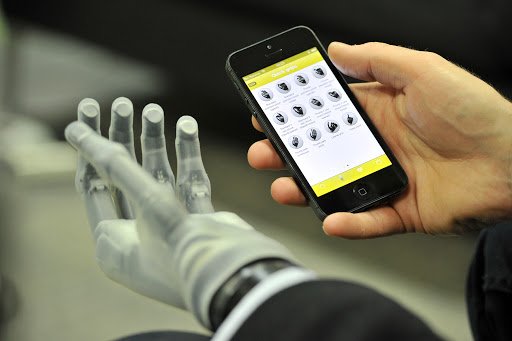
\includegraphics[width=.8\linewidth]{touch_bionics_prothesis.jpg}
	\caption{The i-limb line of hands are developed by Touch Bionics, its proposal of easy adaptability and versatility offer great comfort for users. Offering a range of commands that can be changed in a companion application.} \label{fig_prothesis}
\end{figure}

\section{Importance of Information in \ac{EMG} Signal}

The search and processing of information is a complex cognitive process that requires the identification of extraction and organization of relevant information. However, with the evolution of cloud computing, deep learning-based classification techniques have grown a lot, as they see performing better than conventional Machine Learning techniques. This increase in the use of Deep Learning techniques often makes it often not necessary to understand the problem or delimit its edges.

This approach creates a problem, as there was no learning from the process. The knowledge of how to solve the problem is still lacking and the result is dependent of the neural network, that is trained to do only one task. This dependency creates the need for networks as complex as the first to solve similar problems.

In 1948, Claude Shannon published an article called Mathematical Theory of Communication~\cite{mainreferences}{C.E.Shannonvol.27pp.JulyOctober1948}. In this article, Shannon describes how information can be communicated by different elements of a system. Shannon shows how signs and noises relate and how the ability to separate it to extract information from the data is crucial to the communication process.

Information is usually measured in bits and, a bit of information allows the choice of two equally likely alternatives. As an example, we have the posting of a currency, when revealing the result, a bit of information is generated.

The information theory has its own sets of terms. A message is an orderly sequence of symbols. A message composed of symbols \(\textbf{s} = (s_1, ..., s_n) \) is encoded by a function \( \textbf{c }= f(\textbf{s})\) in a sequence of codes \(\textbf{c} = (c_1, ..., c_m)\), where the number of symbols or codes are not necessarily the same. These codes are transmitted over a communication channel to produce outputs \(\textbf{y} = (y_1, ..., y_k)\) that are decoded to rebuild the message \(\textbf{s}\).

\begin{figure}[h]
	\centering
	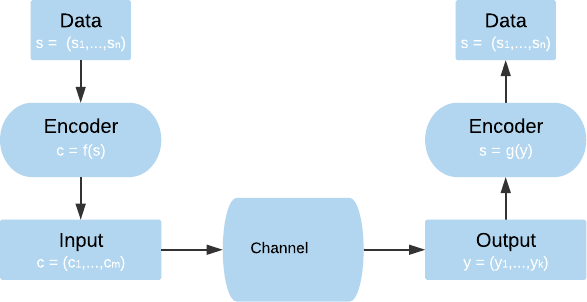
\includegraphics[width=.8\linewidth]{communication_diagram.png}
	\caption{Discrete noiseless channel. The data from a source is  encoded and transmitted thought a communication channel. At the ohter side, a receiver decode the  codeword and recover the original message.} \label{fig_prothesis}
\end{figure}

\section{Introduction to Entropy}

Also according to Shannon~\cite{mainreferences}{shannon1949mathematical}, For mathematical definitions of information to be useful, they must obey the following properties:
\begin{enumerate}
\item \textbf{Continuity:} The total information associated with a result increases or decrements continuously, according to the change in the probability of the result.
\item \textbf{Symmetry:} The total information associated with a sequence of results does not depend on the order in which the results happen.
\item \textbf{Maximum value:} The total information with a result set cannot increase if these results are equally likely.
\item \textbf{Addition:} The information associated with a result set is obtained by adding the information of the individual results.
\end{enumerate}

\subsection{Surprise and Entropy}

The more unlikely a result, the more surprise it is taken with your observation. Then the total surprise associated with a result increases if the probability of the result decreases. Then, to satisfy the condition of aditivity, Shannon used the logarithm of \(1/p(x)\).  This is known as Shannon information of \(x\), i.e. Shannon information is a measure of surprise. The average surprise of a variable \(X\), with a distribution \(p(X)\) is called entropy of \(p(X)\) and is represented by \(H(X)\).

\begin{equation} \label{eq:re}
H(X) \approx \frac{1}{n} \sum_{i=1}^{n} log(\frac{1}{p(x_i)})
\end{equation}

Basically, entropy is the measure of uncertainty. When uncertainty is reduced, information is gained. Therefore, if the uncertainty of a variable \(X\) is summarized by its entropy \(H(X)\), if the value of \(X\) is revealed, the total information gains is, on average, exactly equal to entropy.

If there are consecutive and related values, then they do not provide independent information. In this case the sequence has less entropy than the sum of the individual entropy calculated with the \autoref{eq:re}. Thus, Shannon's theorem applies not only to independent element sequences, but also to structured sequences that have dependencies between their elements.

\section{Entropy and signal \ac{sEMG}}

The \ac{sEMG} signal, like all natural signals, is a diluted signal, that is, a signal that has a lot of data and little information. Moreover it is a sign in which each sampling sequence has a high degree dependence between its values.

The figure \ref{fig_semg} exemplifies the \ac{sEMG} signal measured on the forearm for close the hand movemnet. The movement was repeated three times, for three seconds with a three-second interval between the movements. As we can see from the figure, the three repetitions led to different patterns in the graph. 

\begin{figure}[h]
	\centering
	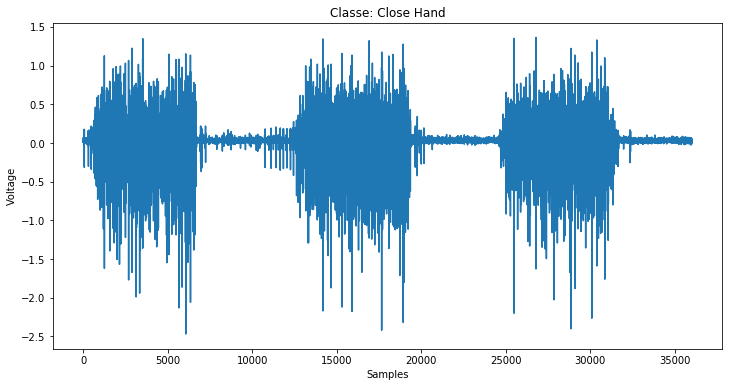
\includegraphics[width=.8\linewidth]{sEMG_signal_close_hand.png}
	\caption{The \ac{sEMG} signal, the vertical axis represents the amplitude and the horizontal axis represents the samples.} \label{fig_semg}
\end{figure}

This occur because in each movement, different motor units are recruited, generating different electrical signals. Other factors that alter the measurement are the displacement of the sensors, sweat and muscle fatigue. One way to mitigate these effects is to acquire information a priori. Where each piece of information extracted facilitates the future classification of the signal.

With the use of a state machine, the possible movements, given a posture for the hand, were mapped and the intersection with the cluster generated a list of possible movements, greatly facilitating the classification of the EMG signal.

\subsection{Real-time processing}

Radhika Menon, et al~\cite{mainreferences}{RadhikaMenonStudentMemberIEEEGaetanoDiCaterinaHebaLakanyMemberIEEELykourgosPetropoulakisBernardA.ConwayJohnJ.SoraghanSeniorMember} shows the impact of the size of the temporal window on the signal classification error \ac{sEMG}. According to this study with very small windows, on average less than 200 ms the classification error increases, since the total information in the window decreases. This makes it very difficult to process in real time that needs windows, in 2011 Peerdeman~\cite{mainreferences}{Peerdeman2011} found that the processing window needs to be less than 300 ms or the delay becomes unacceptable to the user. Instinctively, the need for the decrease of the processing time window is in need for increasing user comfort.

A serious problem caused by the decrease in the time window is the difficulty in defining the end of rest and the beginning of movement. Clustering algorithms were used as a way to get more information about the signal. An \ac{NCA} algorithm was used to reduce the dimensionality of the extracted characteristics and a hierarchical clustering algorithm grouped the closest movements.

The solution to this problem once again presented itself with a decrease in the entropy of the signal. An auto-encoder algorithm was used for anomaly analysis clustering the signal at rest and the motion and then, a simple perceptron classified the result.

\subsection{Extracting signal information}

To extract information from surface electromyography, a technique known as characteristic extraction was used. The signal was divided into windows of 50 ms, where the sEMG signal is analyzed and frequency-based characteristics are extracted, following the main selected resources and finally, the neural network classifies movement.

The extracted characteristics are:
\begin{enumerate}
\item Spectral Moment (\ac{SM});
\item Sample Entropy (\ac{SE});
\item KhushabaSet;
\item Wave Lenght (WL) Frequency);
\item Mean Frequency;
\item Meadian Frequency.
\end{enumerate}

\section{Objective}

\subsection{Main Objective}
To develop an algorithm for a robotic prosthesis using the latest state of the art technologies art of myoelectric prostheses, from a proportional and simultaneous control, which allow posture recognition of the hand joints.

\subsection{Specific Objective}
When obtaining the maximum information from the myoelectric signal, the dimension of the problem is better understood and with that its classification becomes as efficient as possible.

The objective is to use methods of extracting characteristics and classification of patterns in electromyographic signals,  as well as adaptive training for the recognition of hand movements with varying degrees of freedom, thus increasing the comfort of the user and giving naturalness to movement.  Through these methods, a significant improvement was achieved in the pattern recognition process.

\chapter{State-of-the-Art Overview}\label{chap:StateOfArt}

Pattern recognition for the processing of myo-electrical signals has
been the research base for prosthesis control in the last decade~\cite{mainreferences}{Ortiz-Catalan2013}. In addition, the use of
machines have been disseminated in the \ac{EMG} signal analysis area, to aid in the selection of characteristics and classification of the same~\cite{mainreferences}{Duan2016,Huang2005,Khezri2011,Luh2016}. The project also aims to use adaptive training for that new paradigms can be created and the techniques and methods of analysis of the myo-electric signal can be improved.

The use of pattern recognition techniques is of great importance
for the control of myo-electric prostheses, bringing an improvement in the degrees of freedom and their movement beyond the capacity of their sequential control~\cite{mainreferences}{Englehart2003}. Such control typically consists of extracting characteristics of the signal and in the classification of these characteristics of segmented data in the processing signal to control an actuator. The quality of the movement of these prostheses is proportional to the processes of extracting the characteristics of the myo-electric signal and classification of standards.

\begin{figure}[h]
	\centering
	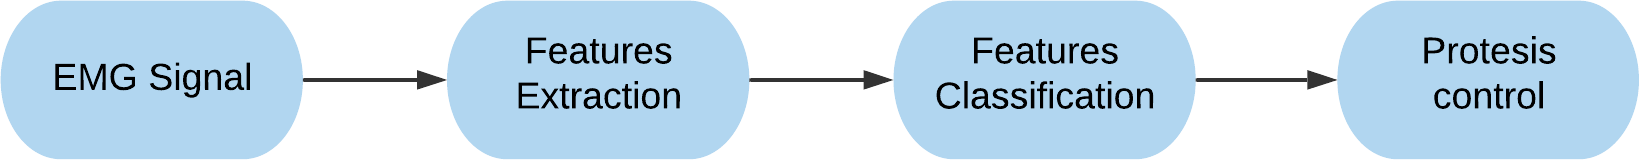
\includegraphics[width=.8\linewidth]{normal_fluxogram.png}
	\caption{The normal fluxogram used for \ac{sEMG} protesis.} \label{fig_norm_flux}
\end{figure}

As already mentioned, most control systems employed in prosthetic hands is sequential control, but recently, a lot of research is being conducted to employ simultaneous control~\cite{mainreferences}{Bennett2017,Dosen2015,RadhikaMenonStudentMemberIEEEGaetanoDiCaterinaHebaLakanyMemberIEEELykourgosPetropoulakisBernardA.ConwayJohnJ.SoraghanSeniorMember,Young2013}. One of the main advantages of simultaneous control of the prosthesis is to approximate the movement of the prosthesis natural physiological, however this leads to an increase in the characteristics necessary to classify the signal, in addition to the interference of the signal from adjacent muscles on the capture of \ac{sEMG}.

\begin{table}[h]
\centering
\caption{State of the art table of sEMG signal analysis.}\label{tab:state_of_art}
\resizebox{\textwidth}{!}{\begin{tabular}{@{}lllll@{}}
\toprule
Reference                      & Class                                                 & Channel                 & Features                                        & Classifier                                  \\ \midrule
(Huang et al. 2005)            & 6 classes of movement                                 & 4 channels              & Gaussian Misture Model (\ac{GMM})                    & \ac{GMM} and Majority Vote                       \\
(Khezri and Jahed 2011)        & 6 classes of movement                                 & 1 channel               & \ac{MAV}, \ac{SSC}, \ac{AR} and \ac{DWT}                            & Neuro-Fuzy                                  \\
(Young et al. 2013)            & 3 degrees of freedom                                  & 6 channels / 8 channels & \ac{MAV}, \ac{ZC}, \ac{SSC} and \ac{WL}                             & Parallel classification strategy            \\
(Bennett and Goldfarb 2017)    & Standardized object relocation and manipulation tasks & 2 channels              & normalized signal                               & Result tables                               \\
(Yang et al. 2011)             & 6 classes of movement                                 & 4 channels              & \ac{DWT}                                             & Fisher criterion, NWFE (Feature projection) \\
(Hartmann et al. 2015)         & 8 classes of movement                                 & 6 channels              & \ac{RMS}, \ac{ZC}, \ac{SSC}, \ac{WL} and \ac{3xCEPS}                     & Linear Discriminant Analysis                \\
(Duan et al. 2016)             & 6 classes of movement                                 & 3 channels              & \ac{RMS} and \ac{DWT}                                     & Wavelet Neuro Network (\ac{WNN})                 \\
(Siu, Shah, and Stirling 2016) & two grab and release sequences                        & 7 channels              & \ac{GMM} and Markov                                  & WPD e Random Forest                         \\
(Luh et al. 2016)              & 16 classes of movement                                & 8 channels              & Four levels of the Daubechies wavelet transform & Neural Network                              \\
(Radhika Menon et al.)         & 7 classes of movement                                 & 128 channels            & \ac{MAV}, \ac{SSC}, \ac{WFL}, \ac{ZC}                               & Linear Discriminant Analysis (\ac{LDA}             \\ \bottomrule
\end{tabular}}
\end{table}

The purpose of this study takes into account the arrangement of several simple networks to extract information and classify the sEMG signal. The figure \ref{fig_final_flux} show the fluxogram used on this study. An autoencoder analyzes the EMG and classifies the state of rest and movement. If the movement starts, a cluster together with the state machine returns the possible movements that may be being executed. The last step is the classifier that chooses the movements among the possible ones for that state.

\begin{figure}[h]
	\centering
	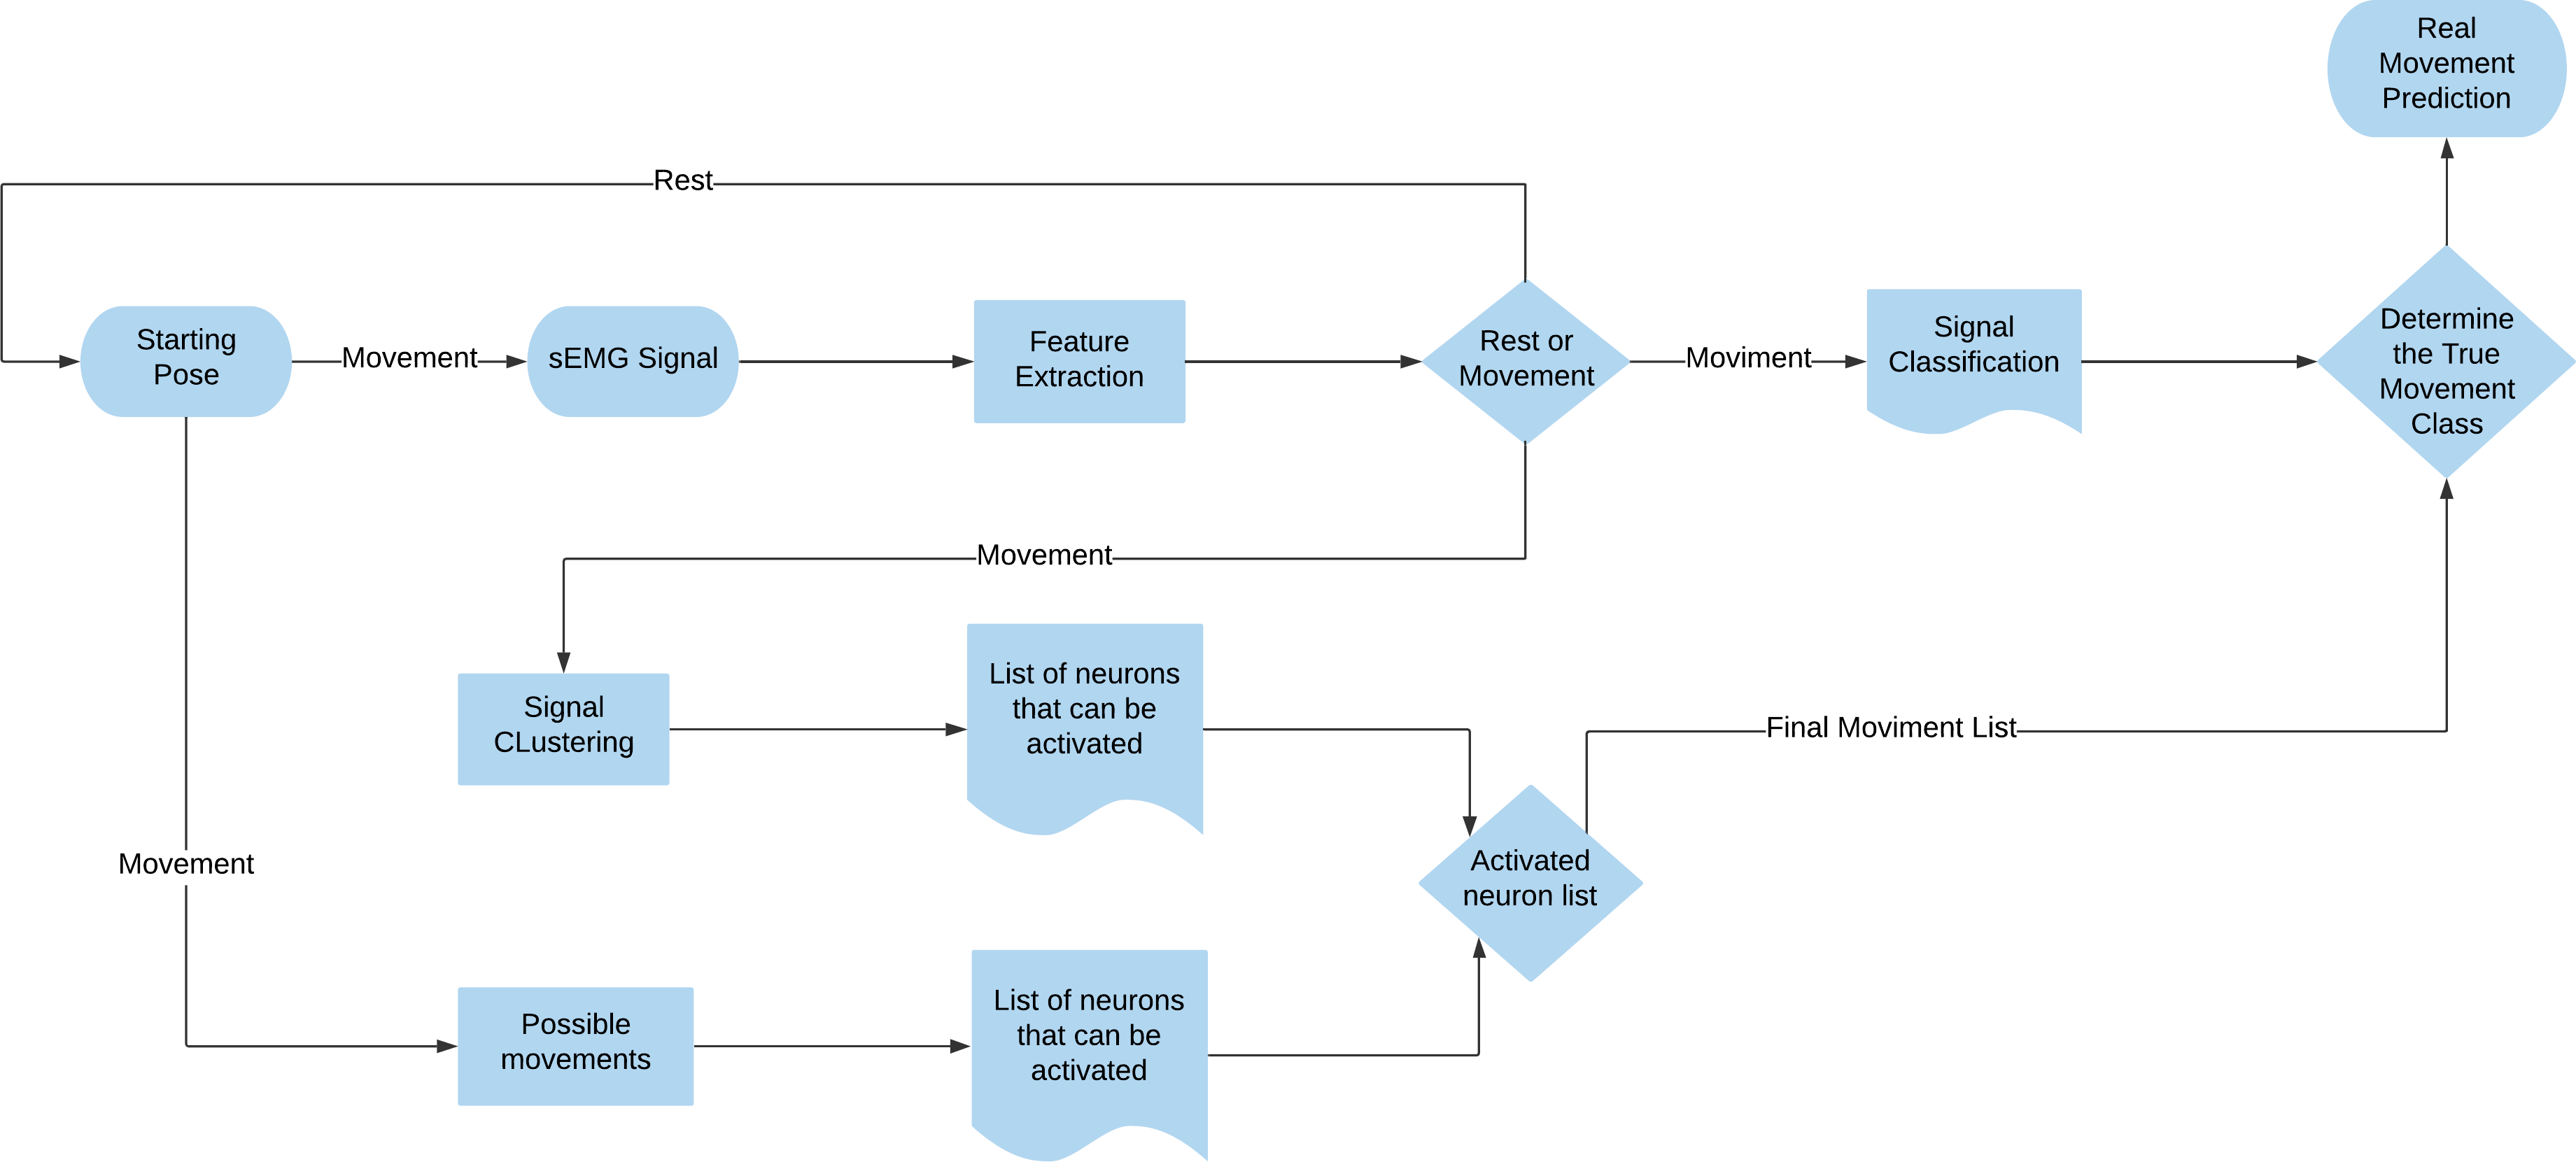
\includegraphics[width=.8\linewidth]{final_semg_classification.png}
	\caption{The proposed fluxogram used for in this study for sEMG classification.} \label{fig_final_flux}
\end{figure}

\chapter{Feature Selection}\label{ch:FS}

\section{Introduction}

Pattern recognition for myoelectric signal processing plays an important role on re-search for prosthetics~\cite{mainreferences}{Ortiz-Catalan2013}. In addition, the application of machine learning techniques has become widespread in the area of surface electromyography (sEMG) signals anal-ysis, to enhance the feature extraction and selection as well the classification of the myoelectric pattern~\cite{mainreferences}{Huang2005,Khezri2011,Duan2016,Luh2016}. Furthermore, the use of pattern recognition brings an im-provement in the degrees of freedom and movement of the prosthesis beyond the ca-pacity of its sequential control~\cite{mainreferences}{Ortiz-Catalan2015}.

In this study, the open source BioPatRec platform was used~\cite{mainreferences}{Ortiz-Catalan2013,Ortiz-catalan2014,Ortiz-Catalan2015}. With a modular and customizable concept, researchers can compare their algorithms easily and efficiently, applying them to control a prosthesis. As advantages, users, by means of this platform, can access the \ac{sEMG} signals database for both sequential and simultane-ous analysis, including quantitative metrics to evaluate the performance of sequential and simultaneous control in a standardized way, as well as to apply methods that the platform provides for feature extraction, feature selection, feature reduction and myoe-lectric pattern classification.

The objective of this work is to analyze new algorithms for feature extraction and selection methods not provided by BioPatRec platform, four additional feature extrac-tion methods were used: the Levinson-Durbin Recursion, the Absolute value of the Summation of the Expth Root Mean, the Mean value of the Square Root and the Abso-lute value of the Summation of Square Root~\cite{mainreferences}{Samuel2017}. Additionally, an unsupervised method for feature selection (UFS) was used~\cite{mainreferences}{Delisle-Rodriguez2017}.

These additions were made for the improvement of the classification of the myoe-lectrical signal to provide a better performance for the simultaneous movement of an upper-limb prosthesis, aiming at increasing the user comfort and giving easing for the movement.

\section{Methodology}

For this study, the “6mov8chUFS” (Untargeted Forearm Simultaneous)~\cite{mainreferences}{Ortiz-catalan2014} database was used, which is freely available on the BioPatRec platform~\cite{mainreferences}{Ortiz-Catalan2013}. The sEMG signal is analyzed, and the features are extracted, following the main features are selected and finally the neural network classifies the movement.

\subsection{BioPatRec Platform}

As previously mentioned, the biomedical signal analysis platform, BioPatRec, was used, using the Multilayer Perceptron Network with backpropagation, already config-ured on the platform for pattern classification.

\subsection{Features Extraction}

In this study were added four time-domain features described below:
\begin{enumerate}[(a)]
    \item The Absolute value of the Summation of the Square root (\ac{ASS})~\cite{mainreferences}{Samuel2017}: This is the first time-domain feature. For calculation of the ASS, the first step is to first execute a full-wave rectification on the sEMG data, this help in retaining the entire energy content of the signal. Next, the integral of the rectified EMG signal is calculated with respect to the current analysis window, as expressed mathematically in Eq. (1)

    \begin{equation}\label{eq:ASS}
    ASS = \left | \sum_{n=1}^{k} (x_n)^\frac{1}{2} \right |
    \end{equation}

    where k represents the analysis window, xn denote the data within the corre-sponding analysis window.
    \item The Mean value of the Square Root (\ac{MSR})~\cite{mainreferences}{Samuel2017}: This is the second time-do-main feature. It provides an estimated measure of the total amount of activity in the analysis window.

    \begin{equation}\label{eq:MSR}
    MSR = \sum_{n=1}^{k} (x_n)^\frac{1}{2}
    \end{equation}

    where k represents the analysis window, xn denote the data within the corre-sponding analysis window.

    \item The Absolute value of the Summation of the expth root (\ac{ASM})~\cite{mainreferences}{Samuel2017} of the data is the third time-domain feature, as shown in Eq. (3). The \ac{ASM} feature pro-vides a comprehensive insight into the amplitude of the EMG signal since it gives an approximate measure of the power of the signal which also produces a waveform that is easily analyzable. This feature contains information from which the amplitude of the rectified EMG signal could be obtained.

    \begin{equation}\label{eq:ASM}
        \begin{split}
        ASM = \left | \frac {\sum_{n=1}^{k} (x_n)^{\exp}}{k} \right | \\
        exp = \begin{cases} 
            {0.50, \:if (n \leq 0 .25\: \times\: k, \:if \:n \geq 0 .75 )}\\
            {0.75 \:otherwise}
            \end{cases}
        \end{split}
    \end{equation}

    The exp. variable can assume one of two possible values (0.50 or 0.75) based on the characteristic of the EMG signal segment under analysis. The \ac{ASM} is therefore determined in the following three steps: first the summation of the expth root of all values in a given analysis window is computed; followed by the mean of the resultant values; and lastly, the absolute value of the resultant mean is evaluated.

    \item The last feature added was the Levinson–Durbin Recursion~\cite{mainreferences}{Zeinali2014}, it is a recur-sive order-update method to the calculation of linear predictor coefficients, it has applications in filter design, coding, and spectral estimation. This method was used to estimate parameters of the \ac{sEMG} signal.
\end{enumerate}

\subsection{Features Selection}
A method based on the Maximal Information Compression Index (\ac{MICI}), and the Entropy Representation (\ac{ER}) was applied for unsupervised feature selection, in order to obtain the best feature sets for the classification~\cite{mainreferences}{Delisle-Rodriguez2017}. Analyzing through the \ac{MICI} to obtain combinations of characteristics with lower value or high redundancy. Those re-dundant features come together with the rejected features, in order to obtain an updated set formed by the features that provide the highest \ac{ER} value during the combination with non-redundant features.

On the other hand, principal component analysis (\ac{PCA}), an orthogonal linear trans-formation, that rearrange the components in the inverse order of variance It is used for dimensionality reduction in the BioPatRec platform as default, as it is a widely used technique.
In that study, \ac{PCA} reduced the 160 features (20 for each channel) to the 64 best features for classification.

Later in chapter\ref{ch:entropy}, new methods of reducing characteristics and dimensionality were tested and evaluated.

\subsection{Neural Network Classifiers}

Despite the existence of a wide variety of different pattern recognition algorithms, the Multi-Layer Perceptron (\ac{MLP}) as a supervised Artificial Neural Network was chosen because of its inherent capacity of simultaneous classification~\cite{mainreferences}{Ortiz-Catalan2013,Ortiz-Catalan2015,AsghariOskoei2007}.

An MLP can be used as a logistic regression classifier, where the input is first trans-formed nonlinearly by a learned transformation. This transformation projects the input data into a space in which it becomes linearly separable. This middle layer is called the hidden layer. A single hidden layer is sufficient to make MLPs a universal approxima-tor. For this study an \ac{MLP} with 3 hidden layers with eleven neurons was used, the transference function was the softmax function.

\subsection{sEMG Database}

As mentioned before, the 6mov8chUFS database was used, and it is available on the BioPatRec platform. This database is formed by 17 subjects, six classes of individual movements were selected, such as hand opening and closing, flexion and extension of the wrist, and prono-supination of the hand, forming 27 possible movements. The signal was measured as follows: 3 seconds contraction time with 3 seconds for relaxation be-tween each repetition, repetitions of each motion. 8 bipolar electrodes (Disposable Ag/AgCl), 1 cm electrode diameter, 2 cm inter-electrode distance for the bipole. Electrodes were equally spaced around the most proximal third of the forearm.

The signal was extracted using overlapped time windows of 0.2 seconds and time increments of 0.05 seconds.

\subsection{Statistical Evaluation}

The tests were performed on seventeen subjects of the original base "6mov8chUFS". First, the BioPatRec feature selection methods were used with and without \ac{PCA}. Finally, the unsupervised feature selection algorithm (\ac{UFS}) was used for reducing features in place of the \ac{PCA}. Thus the tests were completed they were repeated by adding the new characteristic vectors proposed in this study.

The evaluation of the classifier used a cross-validation of 48 trainings with random-ized datasets were per subject and for each algorithm, 24 validation sets, and 49 test sets. For this study was used unitary range normalization.
The BioPatRec provides statistical tools to evaluate the proposed algorithms on the platform, thus, it has a wide variety of metrics~\cite{mainreferences}{Ortiz-Catalan2015} that were used to analyze the results, such as Accuracy (Class Specific), Sensitivity (Recall), PPV (Precision), F1, Specificity (Negative Condition), NPV (Negative Outcome) and Accuracy (Global).

\begin{enumerate}[(a)]
    \item \textbf{Accuracy – Class Specific}
    
    \begin{equation}\label{eq:AccCS}
    AccCS = \frac{absolute \:correct \:predictions}{total \:absolute \:predictions}
    \end{equation}

    \item \textbf{Sensitivity}
    
    \begin{equation}\label{eq:Sensitivity}
    Sensitivity = \frac{TPs}{TPs + FPs}
    \end{equation}

    \item \textbf{PPV}
    
    \begin{equation}\label{eq:PPV}
    PPV = \frac{TPs}{TPS + FPs}
    \end{equation}
    
    \item \textbf{F1}

    \begin{equation}\label{eq:F1}
    F1 = 2 \times \frac{precision \times sensitivity}{precision + sensibility}
    \end{equation}
    
    \item \textbf{Specificity}
    
    \begin{equation}\label{eq:Specificity}
    Specificity = \frac{TNs}{TNs + FPs}
    \end{equation}
    
    \item \textbf{NPV}
    
    \begin{equation}\label{eq:NPV}
    NPV = \frac{TNs}{TNs + FNs}
    \end{equation}
    
    \item \textbf{Accuracy – Global}
    
    \begin{equation}\label{eq:AccG}
    AccG = \frac{TNs + TPs}{TPs + TNs + FPs + FNs},
    \end{equation}

\end{enumerate}

Were TP means true positive, the correct activation; TN is true negative, the correct inactivation; FP is false positive, the incorrect activation; and FN is false negative, in-correct inactivation.

\section{Results and discussion}

It has been shown that the individual movements can be successfully predicted offline using pattern recognition algorithms~\cite{mainreferences}{Ortiz-Catalan2013,Khezri2011,Sensinger2009,Geethanjali2016} and in this study was demon-strated an increase in terms of classification accuracy was achieved when the new fea-tures were used in conjunction with a feature reduction algorithm. Table 1 shows the results obtained using the characteristics present in BioPatRec and the use of \ac{PCA} or \ac{UFS} to reduce characteristics.

\begin{table}[h]
\centering
\caption{Quantitative indicators obtained with the comparison between old features with feature reduction algorithms.}\label{tab:Quantitative indicators}
    \resizebox{\textwidth}{!}{\begin{tabular}{@{}llllllll@{}}
    \toprule
    Features Selection & Accuracy Class & Sensitivity & PPV   & F1   & Specificity & NPV   & Accuracy Global \\ \midrule
    None               & 83.10          & 85.11       & 92.30 & 0.89 & 99.73       & 99.43 & 99.19           \\
    PCA                & 92.74          & 94.78       & 94.78 & 0.95 & 99.80       & 99.80 & 99.61           \\
    UFS                & 90.63          & 92.29       & 95.02 & 0.94 & 99.81       & 99.70 & 99.54           \\ \bottomrule
    \end{tabular}}
\end{table}

Table \ref{tab:Quantitative indicators new features} shows the results obtained using the characteristics present in BioPatRec and those added by this study, in addition to the use of \ac{PCA} or \ac{UFS} to reduce the charac-teristics. As more characteristics are sorted, the MLP begins to diverge, but when se-lecting the most divergent characteristics, through the methods of selecting characteristics, rating the signal becomes easier. The performance of the proposed and the con-ventional methods present in the BioPatRec is shown by the gain in the accuracy and deviation shown in table \ref{tab:Quantitative indicators} and \ref{tab:Quantitative indicators new features}.

\begin{table}[h]
\centering
\caption{Quantitative indicators obtained with the comparison between the new features added to the old features sets with feature reduction algorithms.}\label{tab:Quantitative indicators new features}
    \resizebox{\textwidth}{!}{\begin{tabular}{@{}llllllll@{}}
    \toprule
    Features Selection & Accuracy Class & Sensitivity & PPV   & F1   & Specificity & NPV   & Accuracy Global \\ \midrule
    None               & 82.39          & 83.60       & 95.76 & 0.89 & 99.86       & 99.37 & 99.26           \\
    PCA                & 94.63          & 96.22       & 96.95 & 0.97 & 99.88       & 99.85 & 99.75           \\
    UFS                & 93.50          & 94.71       & 96.68 & 0.96 & 99.87       & 99.80 & 99.68           \\ \bottomrule
    \end{tabular}}
\end{table}

The below figure shows the distribution curves of the experiment, while the blue curve represents the old features the red one represent the experiment with the added features.

The difference between two means divided by a standard deviation for the data is rep-resented with the "d" letter in the graphic.

\begin{figure}[h]
	\centering
	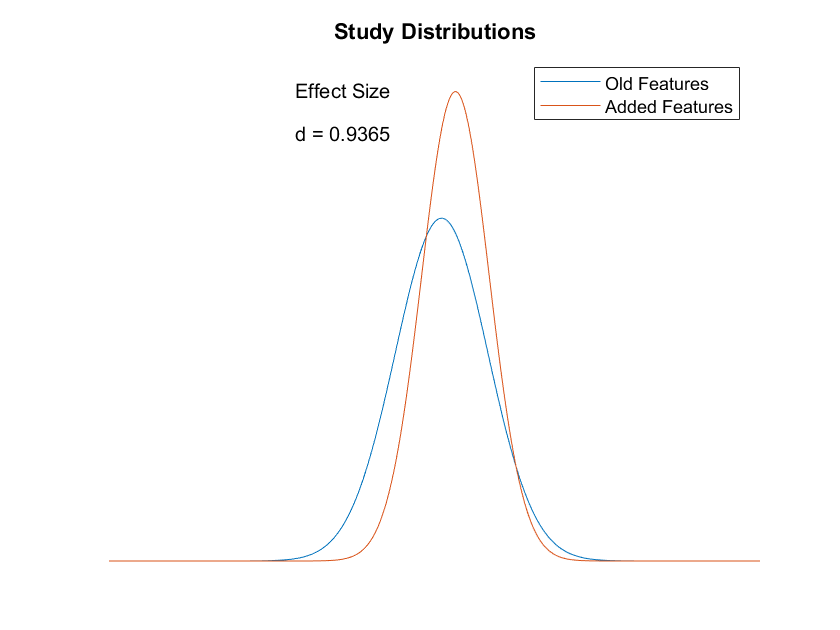
\includegraphics[width=.8\linewidth]{Study_Distributions.png}
	\caption{Distribution of the experiment with the old features and the added features.} \label{fig1}
\end{figure}

According to Cohen and Sawilowsky:
\begin{itemize}
    \item $d = 0.01 \implies very \:small \:effect \:size$;
    \item $d = 0.20 \implies small \:effect \:size$;
    \item $d = 0.50 \implies medium \:effect \:size$;
    \item $d = 0.80 \implies large \:effect \:size$;
    \item $d = 1.20 \implies very \:large \:effect \:size$;
    \item $d = 2.00 \implies huge \:effect \:size$.
\end{itemize}

The experiment was offline, and the mean training and validation time was of 34 seconds and the mean testing time was of 0.004 seconds.

The use of BioPatRec allows a fast and accurate simulation of the pattern recognition algorithms, which streamlines the process of development and testing of theories that will be applied in the control of a myoelectric prosthesis. This platform is being used in this study and it is hoped that it can assist in the development of an adaptive learning pattern recognition system for the control of an upper limb electrical prosthesis. In ad-dition, the fact that the BioPatRec platform is modular allows the study to be better divided into stages, such as signal processing, extraction of characteristics, classifica-tion and the decision-making system of the prosthesis, making the process agiler.

\section{Conclusion}

The addition of the new features in conjunction with the selection algorithms improved the characterization of the myoelectric signal, which will facilitate the decision process for the control of the myoelectric prosthesis. The help of the BioPatRec platform made the work agiler and the statistical metrics helped to evaluate the effectiveness of the algorithms applied in this study. Furthermore, this study showed that simultaneous con-trol can be considered since it improves user comfort. In addition, simultaneous control is required for more natural control of artificial limbs, and pattern recognition has proved to be an excellent means of working with the complexity generated by simulta-neous movement.

\chapter{Autoencoder and Anomaly Detection}\label{ch:AnamalyAnalisys}

\section{Introduction}

An autoencoder is a neural network that is trained to attempt to copy its input to its output. While copying the input to the output may be useless, a high-dimensional data can be converted to low-dimensional codes by training a multilayer neural network with a small central layer to reconstruct high-dimensional input vectors. Using the inner layer, also called latent space, we have a signal with a reduced size, more easily classified.

The \ac{VAE} is a generative model that estimates the Probability Density Function (\ac{PDF}) of training 
data. By training the model to recognize the \ac{sEMG} signal it will assign a high probability value to a motion class, while the noise will receive a low probability value\cite{mainreferences}{Welling}.

The \ac{VAE} model can also sample examples of the PDF learned, thus generating new examples similar to the original data set. But it is important to emphasize that \ac{VAE} is not a way of training generative models, but rather that the generative model is a component of \ac{VAE}, generally being a deeply latent Gaussian model\cite{mainreferences}{Rezende2014}.

In the figure \ref{fig2} are the steps to summarize the operation of a \ac{VAE}. On the left side we have the model definition:

\begin{enumerate}
    \item  Let \(q(z|x)\) be defined as how the signal is encoded into a distribution over the latent space;
    \item  Let z be A latent vector sampled from \( q(z|x) \), \(z\) will contain the information describing \(x\). The decode of it is represented as \( p(z|x) \);
    \item  \(z\) is decoded as a signal.
\end{enumerate}

On the right side we have the loss:

\begin{enumerate}
    \item Reconstruction error: the difference between the output and the input.
    \item \( p(z|x)\) should be similar to the prior (multivariate standard Gaussian).
\end{enumerate}

The \ac{VAE} generating coefficient appears by directly sampling the latent vector from the prior distribution and decoding it into a noisy representation of \( x \)\cite{mainreferences}{Welling}.

\begin{figure}
	\begin{center}
	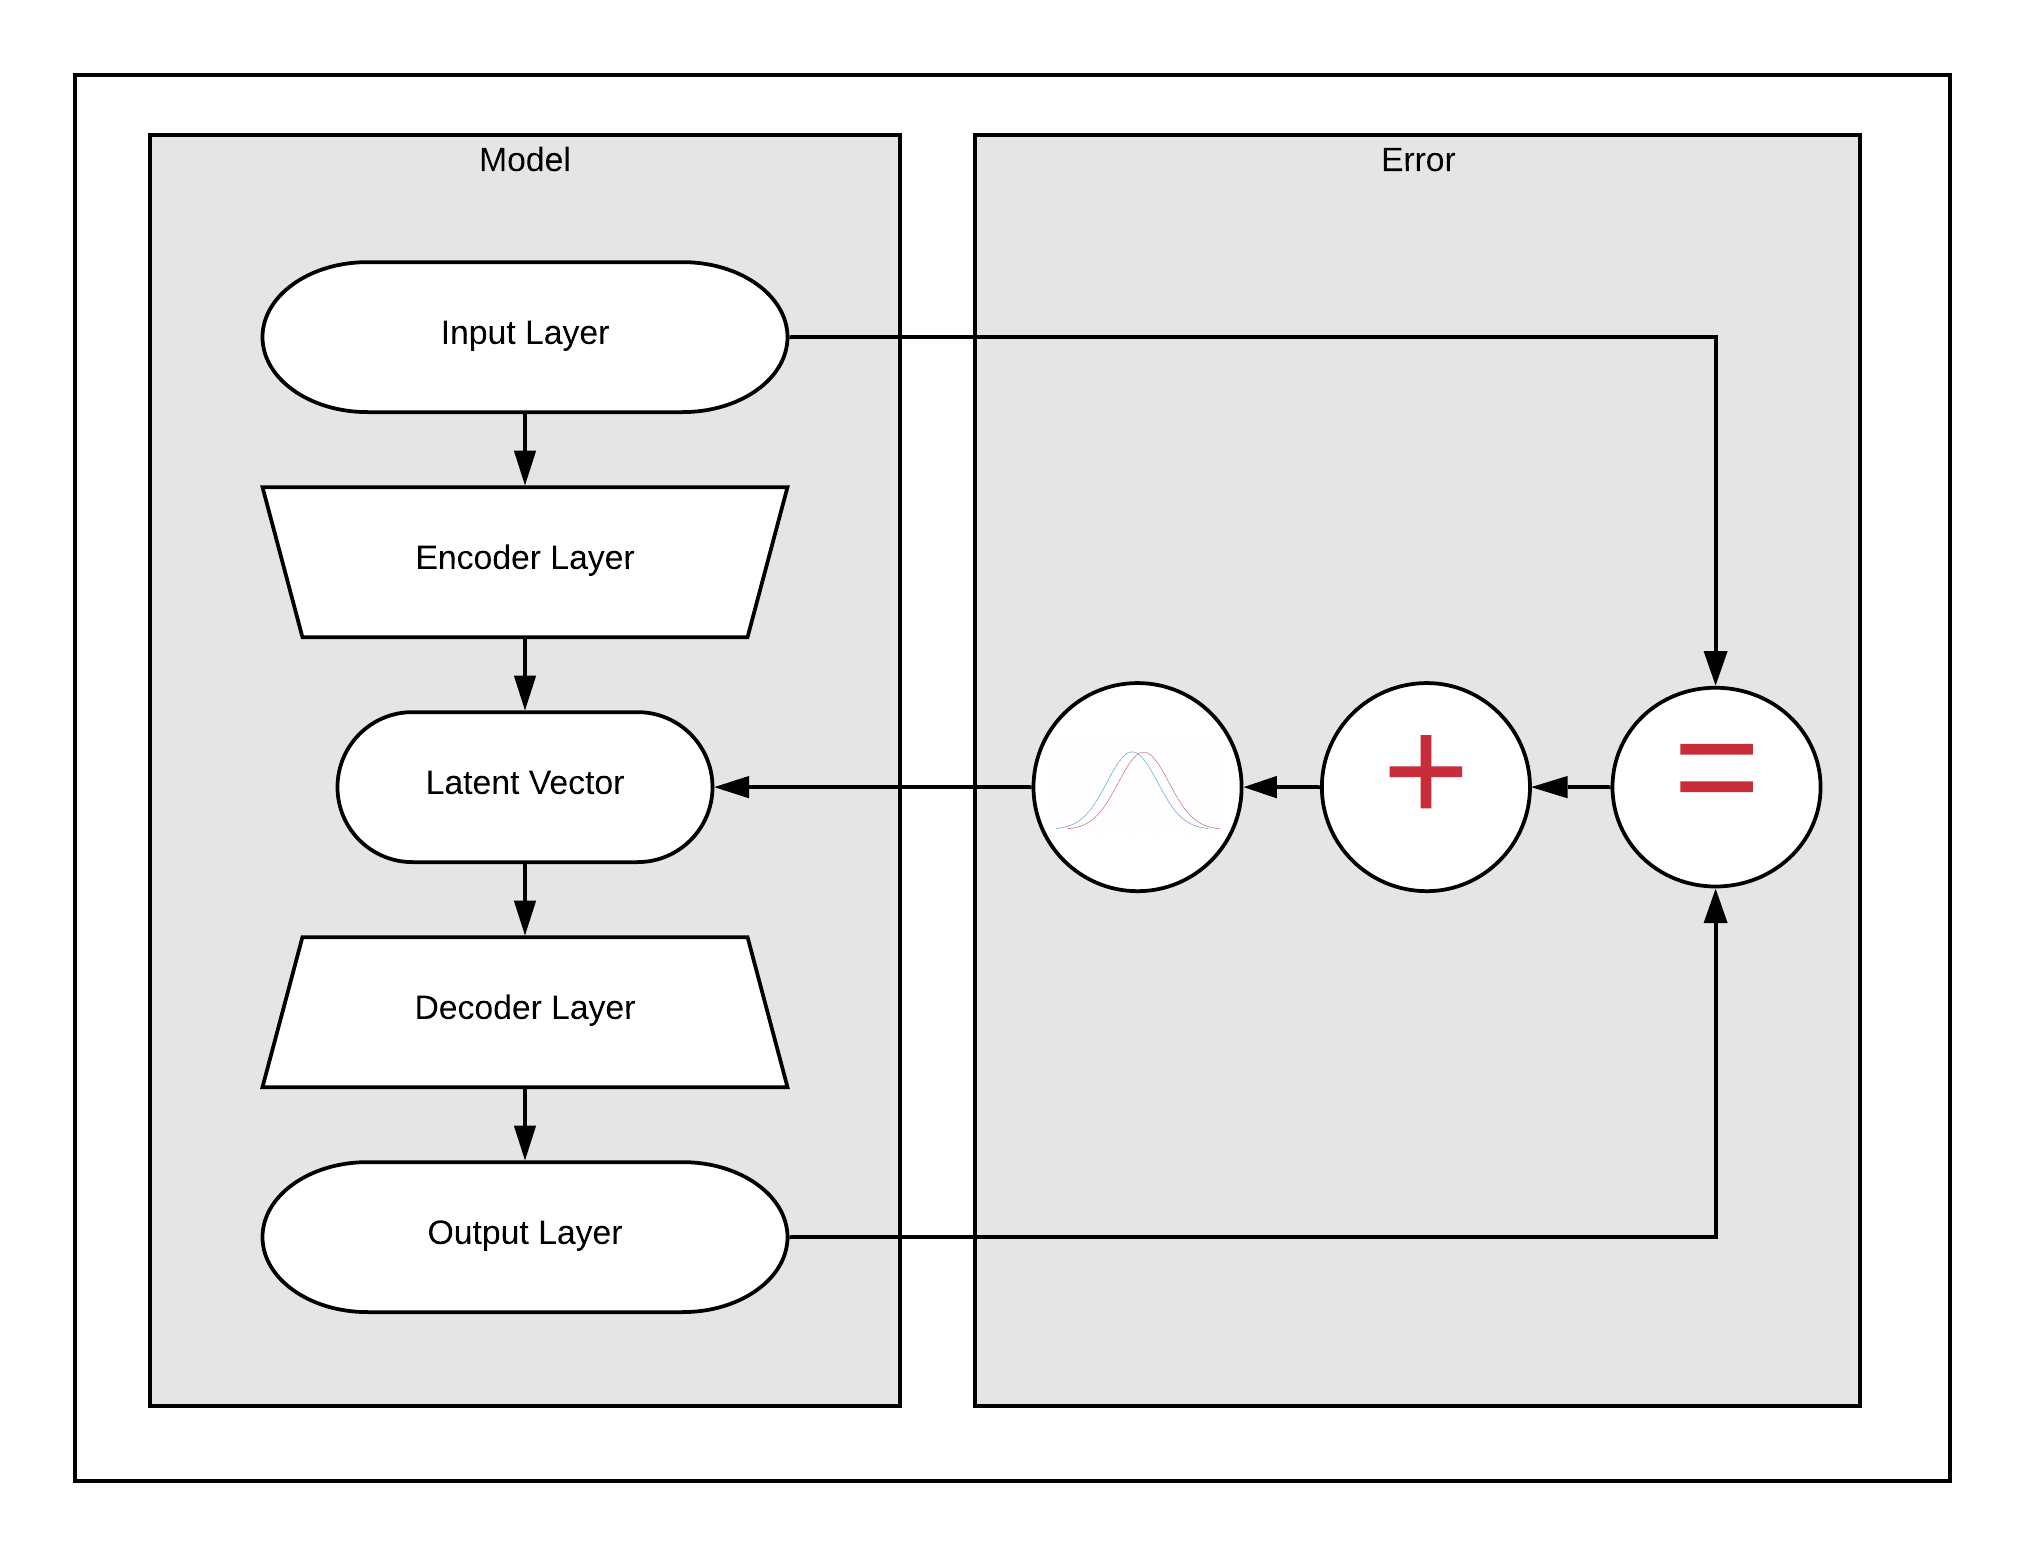
\includegraphics[width=.8\linewidth]{VAE_Diagram.png}
	\end{center}
	\caption{Flowchart of a variational autoencoder} \label{fig2}
\end{figure}

%\hfill mds
 
%\hfill July 26, 2019

\subsection{Model specification}

\subsubsection{Encoder layer}

In Bayesian modeling, the distribution of observed variables is governed by latent variables. The latent variables are extracted from a previous density \( p(z)\) and related to the observations through the probability \( p_\theta(x|z)\). Deep latent gaussian models (DLGMs) are a general class of models where the observed variable is governed by a latent variable hierarchy, and the latent variables at each level of the hierarchy are Gaussian a priory\cite{mainreferences}{Rezende2014}.

Normally, in the \ac{VAE}, a Gaussian distribution is used to sample the latent space.

\begin{equation}
    p(z)=N(0,I) 
    \label{eq1}
\end{equation}


In this way, each local latent variable is related to its corresponding observation through the likelihood \( p_\theta(x|z) \), which can be seen as a probabilistic decoder. Using a hidden smaller representation \(z \), it decodes it into a distribution over observation \(x \).

\subsubsection{Decoder layer}

The decoder is another neural network. Its input is the latent vector \( z \), generates the parameters for the probability distribution of the data and has weights and biases \( \theta \). The decoder is denoted by \( p_\theta (x|z)\). The probability distribution is a multivariate Gaussian.

The loss function of \ac{VAE} is the negative log-likelihood with a regularizer. Since it is not possible to
generalize the global representation shared by all data points, we can decompose the loss function into terms
that depend only on a single data point \( l_i \). The parameters are typically the weights and biases of the
neural networks represented as \( \theta \) and \(\phi\). The total loss will then be represented by the sum of
all losses \( l_i \) for all data points. The loss function \( l_i \) for the data point \( x_i \) is:

\begin{equation}
    l_i(\theta,\phi) = \mathbf{E}_{z~q_\theta}(z ∣| x_i)[log(p_\phi(x_i |∣ z))] +\mathbf{KL} (q_\theta(z |∣ x_i)∣|| p(z))
    \label{eq2}
\end{equation}

The first term represent the reconstruction loss, and has the form of a negative log-likelihood of the i-th data point. The expectation is taken with respect to the encoder’s distribution over the representations. This term encourages the decoder to learn how to reconstruct the data. If the decoder’s output does not have similarity with the data, statistically the decoder parameterizes a likelihood distribution that does not place much probability mass on the true data. Poor reconstruction will incur a large cost in this loss function.

The second term is a regularizer. This is the Kullback-Leibler divergence between the encoder’s distribution \(q_\theta(z|x)\) and \(p(z)\). This divergence measures how much information is lost when using \(q\) to
represent \(p\), in other words, the divergence of the approximate from the true posterior.

\subsubsection{Inference Network}

An inference network is a flexible construction for parameterizing approximating distributions during inference\cite{mainreferences}{Dayan1999}, and it is used on VAE\cite{mainreferences}{Rezende2014, Welling} to infer the optimal values of the latent variables given observed data, or to calculate the posterior \(p(z∣|x)\). By modeling the true
distribution P(z|X) using simpler distribution that is easy to evaluate, e.g. Gaussian, and minimize the
difference between those two distribution using KL divergence metric, as in \ref{eq2}, which tells us how difference it is \(p\) and \(q\).

\subsection{Anomaly Detection}
The use of auto-ponder for anomaly detection is already common in the area of artificial intelligence~\cite{mainreferences}{Vostrova1986,Zong2018,Aytekin2018}. In this study, a variational autoencoder was used to detect the onset of movement, which is otherwise confused with the resting state.

The test of the usability of the auto-encoder was done for the classification of the 26 classes of movement of the database, it was later retrained to detect the change of the resting state.

\section{Methodology}

\subsection{Database}
In this work the "6mov8chFUS" database made available with the BioPatRec platform\cite{mainreferences}{Ortiz-Catalan2013} was used. The “6mov8chUFS” database consists of 17 patients, with six individual movement classes selected, such as opening and closing the hand, flexion and extension of the wrist, and prono-supination of the hand, forming 27 possible movements.

The signal was measured as follows: 3 seconds of contraction time with 3 seconds for relaxation between each repetition, repetitions of each movement. 8 bipolar electrodes (disposable Ag / AgCl), 1 cm of electrode diameter, 2 cm of inter-electrode distance for the bipolar. Electrodes were equally spaced around the proximal third of the forearm.

\subsection{VAE Algorithm}
A simple Variational Autoencoder was used for the anomaly detection phase. The encoder stage was compose of three dense layers. The first one have 32 neurons, the second 16 neurons and the third 8 neurons. The sampling inference, which characterizes the variational autoencoder, is made on top of the last layer of the encoder step, which has 8 neurons. All layers in this phase have the Rectified Linear Unit (ReLU) as the activation function.

The decoding stage is the reverse of the encoding. It starts with 8 neurons in the first layer, 16 neurons in the second and 32 neurons in the last. The first two layers have ReLU as the activation function and the third layer, the sigmoid as the activation function.

\begin{figure}[h]
\centering
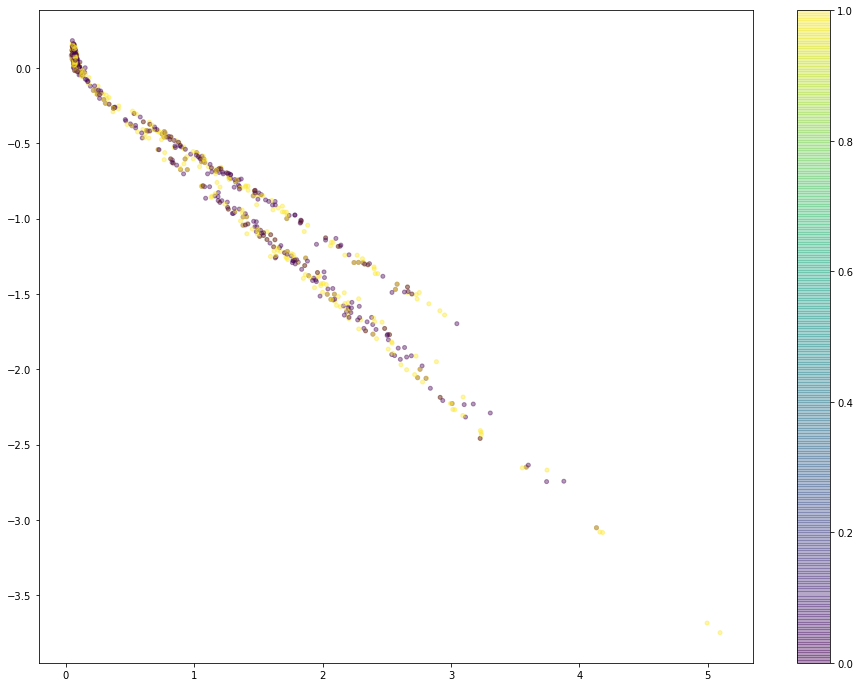
\includegraphics[width=.8\linewidth]{latent_space_vae.png}
\caption{The latent space representation created by te Variational Autoencoder} \label{fig_lat_space}
\end{figure}

The figure \ref{fig_lat_space} is the dimensionless values of the autoencoder trained with two neurons in the latent layer. The figure represents the representation of the anomalies found when the patient starts to move. With that output of the latent space, a simple perceptron network is used to detect whether the patient is moving or resting.

\section{Results}

In this experiment, a 0.01s window (10 samples) was used. With this window size, normal classification methods cannot accurately classify the movements classes or even differentiate the resting state of movement. Through the use of auto-encoder as an anomaly detector, it was possible to determine the moment when the movement really started.

The figure \ref{fig_lat_space_rep} is the representation of the difference between the rest movement state in the latent space of the variational autoencoder. For the construction of the image the latent space was dimensioned with 4096 neurons. The output of the neurons has been scaled to a 64 by 64 square shape and the image was made.

\begin{figure}[h]
    \begin{center}
	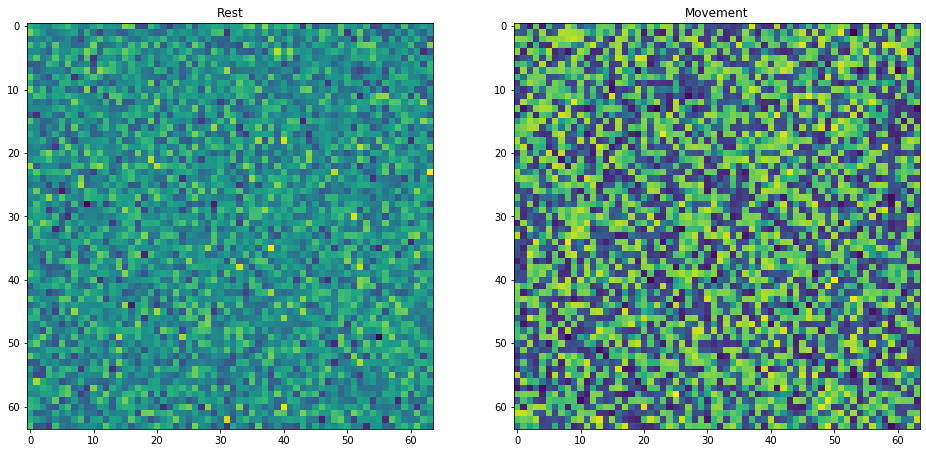
\includegraphics[width=.8\linewidth]{latent_space_as_image.png}
	\end{center}
	\caption{A expanded latent space, to represent the diference between the rest and the rest and the movement state. In this image the latent space was dimensioned to be 64 x 64 to facilitate the diference visualization.} \label{fig_lat_space_rep}
\end{figure}

It is worth remembering that, although the detection of the anomaly only needed eight neurons to be able to perform successfully, the representation of the latent space needed to be enlarged so that the difference was visible to our eyes.

\section{Conclusion}

The results obtained demonstrate the feasibility of the variational autoenconder as an anomaly detector for the \ac{sEMG} signal. Furthermore, by separating the resting state from the other classes of movement, the entropy of the system is reduced, facilitating the future classification of the other classes of movement.

By using \ac{VAE}, which is specialized in separating classes in their latent space, movement detection has been simplified and its computational cost has been greatly reduced. Although the training was done only using the offline signal, simulating the acquisition of the signal online proved to be extremely efficient.

In this study, the auto encoder was used only as an anomaly detection instrument, but its use is not limited to that. As shown in figure ~\ref{fig_lat_space_rep}, the autoencoder can be used to increase the separation between classes just by increasing the size of the latent space. This technique can be used in further studies to improve the system accuracy.

\chapter{Entropy}\label{ch:entropy}

\section{Introduction}

The \ac{EMG} signal varies according to the posture, position, and force applied by the person that is performing a muscle contraction. Therefore, to have perfect control of a prosthesis, extensive training with a myoelectric unit is required. However, as these prostheses have a high cost investment, it is often not possible to offer longterm training for their use.

One of the difficulties regarding \ac{EMG} signal processing for use in prosthesis control is the need for real-time processing. This creates the need for ever-smaller time windows that, in turn, have less signal information, which limits the amount of information that can be extracted from them.

In the last few years, deep learning techniques have become increasingly used, but the more complex the applications are, the more complex the neural networks become. However, the more parameters the network has, the higher the chance of having over-fitting, which causes considerable deterioration to the network’s generalization capacity. Otherwise, if the neural network has few parameters, it will probably not be able to represent the data accurately. Notably, the best way to achieve generalization is to seek a balance between training error and network complexity~\cite{mainreferences}{LeCun1990,Zhang2019}.

In the tasks of biosignal classification, there are frequently too few biomedical signal samples to allow for the achievement of good results with deep learning~\cite{mainreferences}{Sarunas1991}. Another problem associated with deep learning is the cost of training processing, which demands specific hardware and high computational cost due to the complexity of the current neural networks architectures~\cite{mainreferences}{Zhang2019}. This thesis suggests extracting maximum signal information before signal classification as a method to reduce the system complexity and create redundancy for the classification and thereby managing to decrease the time window for the real-time processing of the signal. One of the steps of the algorithm proposed includes the development of a pipeline that extracts a priori information from the EMG signal by computing the current hand and forearm postures and the similarity of the EMG signals from the forearm.

As mentioned before, one way to ensure entropy reduction (information gain) is to obtain a priori information~\cite{mainreferences}{shannon1949mathematical}. The starting position of the hand and forearm provide a great deal of information to the classifier as it restricts possible
movement classes. For this purpose, a state machine~\cite{mainreferences}{AsghariOskoei2007} that counts the possible movements from the initial classes was
created. This state machine reduced by just over three times the number of classes to classify, improving the classification
of the system.

A second method used in this work for entropy reduction, was the classification of signals by similarity. Therefore, a Hierarchical Agglomerative clustering (\ac{HCA}) technique was selected. In this technique, each data point is considered an
individual cluster. At each iteration, using distance, a similar pair of clusters are merged as they move up the hierarchy,
until there is a formation of one cluster or K clusters.

The proposed methodology led to a substantial decrease in the size of the temporal window used for sEMG signal processing. Besides, there was also an improvement in the generalization and processing speed due to the simplification of the model used for classification.

This chapter is organized as follows: Section II shows a detailed explanation of the algorithms used. The results are listed in Section III, which also presents a detailed analysis of the experiment. Finally, there is a conclusion, where the results are summarized.

\section{Methodology}

\subsection{The Pipeline}
Initially, there is an estimation of the original positions of the hand and forearm. The possible movements are checked by analyzing the state machine; these two steps lead to a list of values associated with the neurons that are activated in the final layer of the classifier.

\begin{figure}[h]
    \begin{center}
	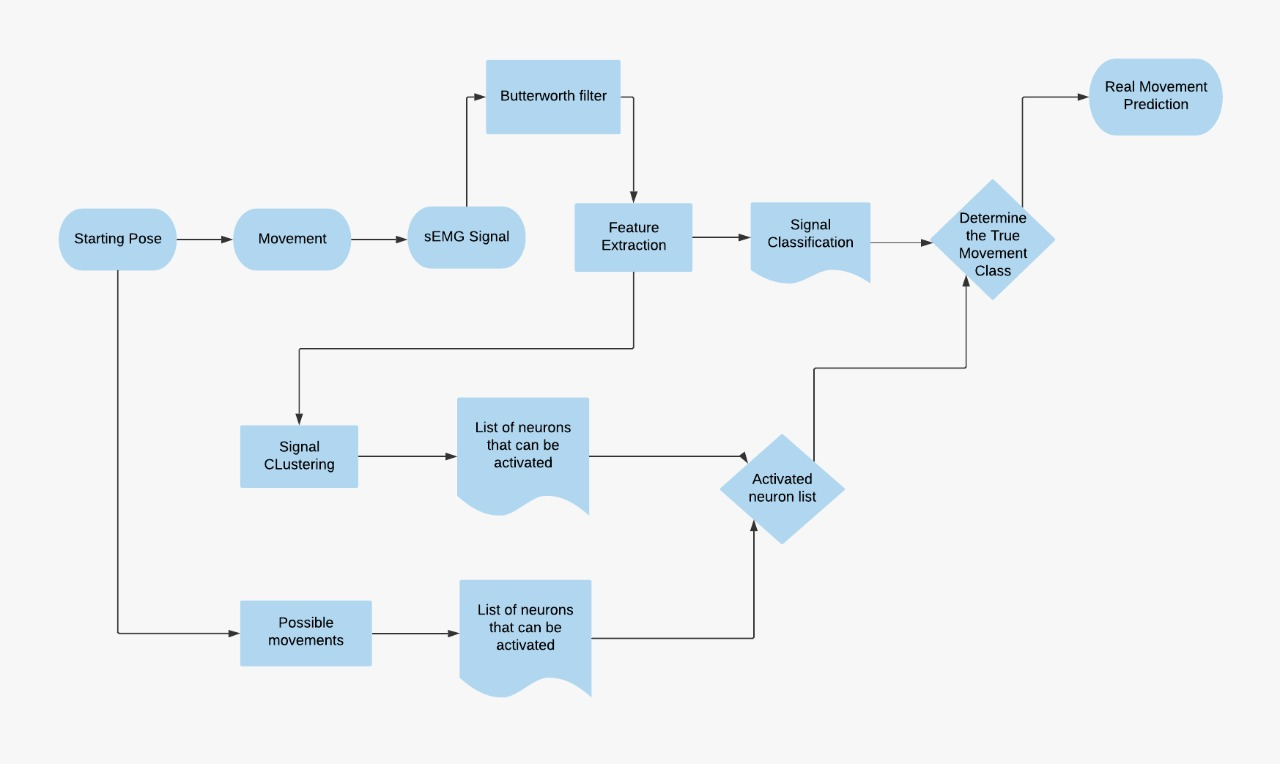
\includegraphics[width=.8\linewidth]{sMEG_Classification_Fluxogram.png}
	\end{center}
	\caption{Pipeline representation: the algorithm begins at a starting position; the \ac{sEMG} signal is measured and pre-processed to help to determine the movement intention; with these two information pieces, the possible next movements are determined as well as the cluster to which the class belongs; finally, the algorithm yields the movement intention.} \label{fig_class_fluxo}
\end{figure}

The second step is processing the signal with the Butterworth filter, followed by the feature extraction and standardization of the data. Furthermore, a reduced space transform created by the \ac{NCA} algorithm is applied, and the signal is ready for the classification and clustering algorithms. This transformation reduces the vector of characteristics from 36 to 25 dimensions.

The third step for signal classification is to find the group to which the analyzed window belongs. The \ac{HCA} clustering algorithm will provide a new list of activated neurons in the classifier. In the \ac{HCA} algorithm, each observation starts in its cluster, and the algorithm merges pairs of clusters when one moves up the hierarchy. The intersection between the state machine-generated list and the cluster generates the final list of neurons that can be activated.

The last step is the signal classification by the MLP and the multiplication of the result by the list generated in the previous step. The image below shows the value of neurons before and after applying the list of neurons to be used.

\subsection{Database}

The "6mov8chUFS" database~\cite{mainreferences}{Ortiz-catalan2014} consists of 17 patients, with six individual movement classes selected, such as opening and closing the hand, flexion and extension of the wrist, and prono-supination of the hand, forming 27 possible movements. The signal was measured as follows: 3 seconds of contraction time with 3 seconds for relaxation between each repetition, repetitions of each movement. 8 bipolar electrodes (disposable Ag / AgCl), 1 cm of electrode diameter, 2 cm of inter-electrode distance for the bipolar Electrodes were equally spaced around the proximal third of the forearm.

The algorithm was tested with the "6mov8chFUS" database, made available by BioPatRec platform~\cite{mainreferences}{Ortiz-Catalan2013}. Also, with the help of the BioPatRec platform, an analysis was made using seventeen characteristics. With the use of principal component analysis (\ac{PCA}) the four best characteristics for the execution of the algorithm were selected. The number of features was chosen to take into account the speed of the information processing, which needed to be as fast as possible to create the most natural movement possible.

\subsection{Movement Classes}

The movement classes used in the "6mov8chUFS" database are listed as follows:

\begin{enumerate}
    \item Open Hand
    \item Close Hand
    \item Flex Hand
    \item Extend Hand
    \item Pronation
    \item Supination
    \item Open Hand + Flex Hand
    \item Close Hand + Flex Hand
    \item Open Hand + Extend Hand
    \item Close Hand + Extend Hand
    \item Open Hand + Pronation
    \item Close Hand + Pronation
    \item Open Hand + Supination
    \item Close Hand + Supination
    \item Flex Hand + Pronation
    \item Extend Hand + Pronation
    \item Flex Hand + Supination
    \item Extend Hand + Supination
    \item Open Hand + Flex Hand + Pronation
    \item Close Hand + Flex Hand + Pronation
    \item Open Hand + Flex Hand + Supination
    \item Close Hand + Flex Hand + Supination
    \item Open Hand + Extend Hand + Pronation
    \item Close Hand + Extend Hand + Pronation
    \item Open Hand + Extend Hand + Supination
    \item Close Hand + Extend Hand + Supination
\end{enumerate}

\subsection{Feature extraction}

In order to reduce signal noise, the first step in extracting features was to use a sixth-order bandpass Butterworth filter, 80-450Hz. Additionally, a time window for sampling the signal is selected. In this study, the sampling frequency of the sEMG was 2000 Hz, with a 0.01s window (i.e., ten samples per window).

This stage was subdivided into two steps:

\begin{enumerate}

    \item \textbf{Selection of characteristics:} to extract information from the signal four frequency domain features were used~\cite{mainreferences}{Jose2018}:
    \begin{itemize}
    	\item  Spectral Moment;
    	\item  Waveform Length (acumulative changes in the length);
    	\item  Mean;
    	\item  Median;
    \end{itemize}
    \item \textbf{Dimensional reduction:} (\ac{NCA})~\cite{mainreferences}{Phinyomark2013} allowed for the dimensional reduction by helping to select the most significant features of the signal. \ac{NCA} is a supervised learning algorithm for distance metric learning. It learns a linear transformation (of input data) that maximizes, in the transformed space, the average leave-one-out classification performance.
\end{enumerate}

The figure \ref{fig_dim_reduction} shows the study made to select the best dimensionality reduction algorithm. The methods were tested with a \ac{KNN} with k =3, the method was select base on the accuracy of the knn. The plots represent the features on the dimensionality reduction algorithm space, therefore they don't have dimensions.

\begin{figure}
\begin{center}
    \subfloat{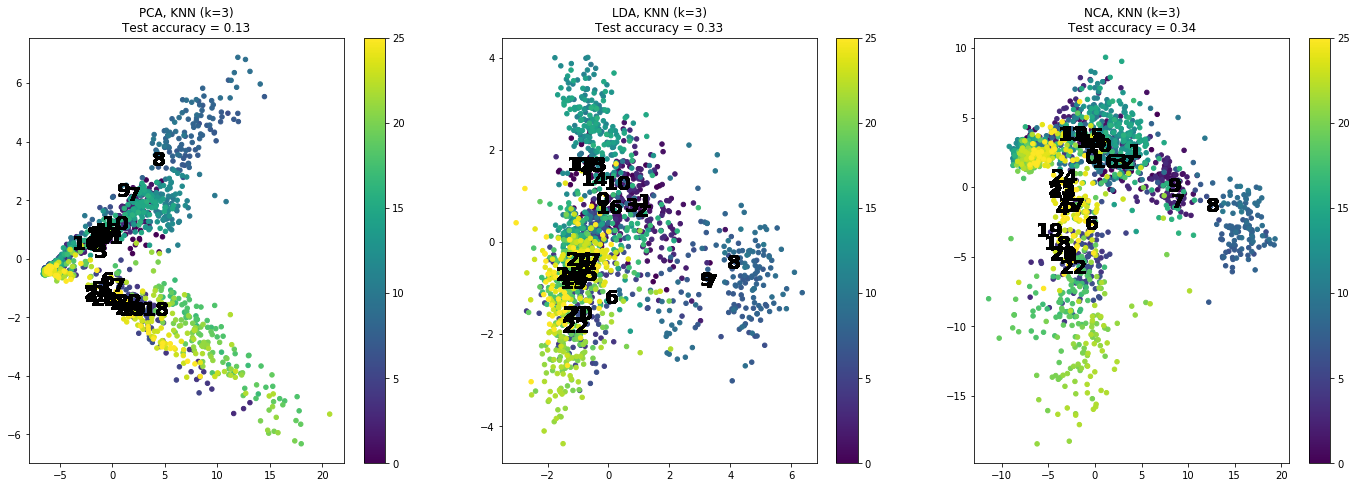
\includegraphics[width=.7\linewidth]{clustering_smg_a.png}} 
    \subfloat{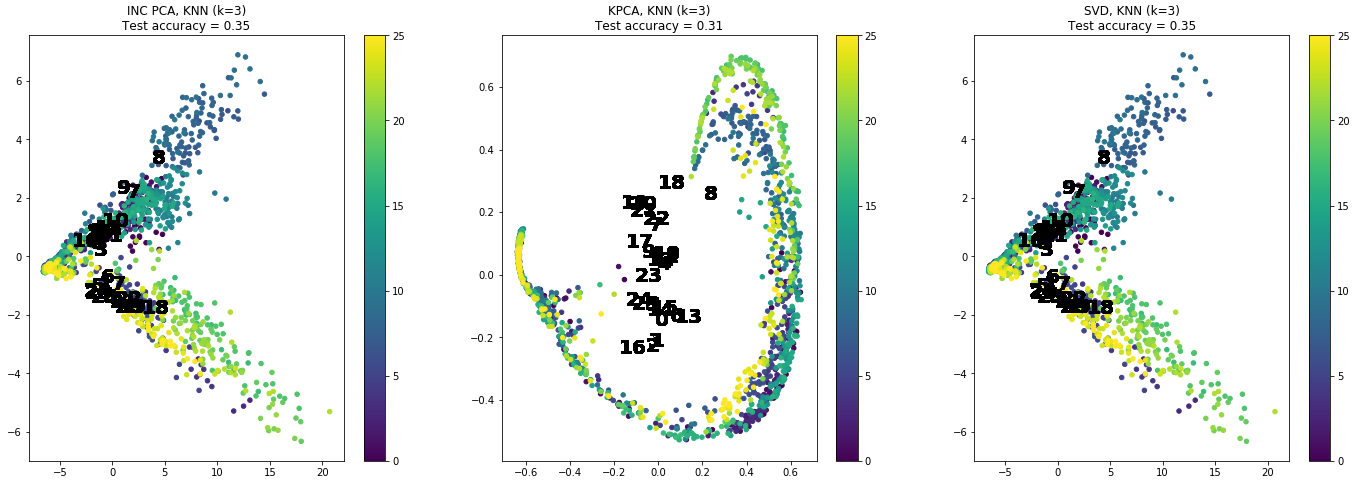
\includegraphics[width=.7\linewidth]{clustering_smg_b.png}}
    \subfloat{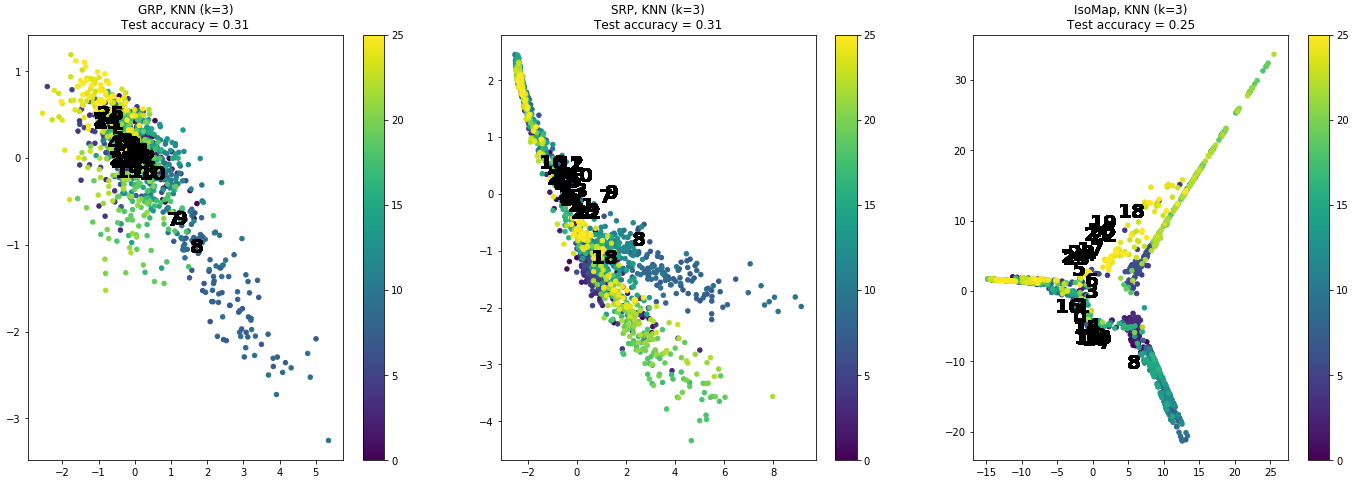
\includegraphics[width=.7\linewidth]{clustering_smg_c.png}}
    \subfloat{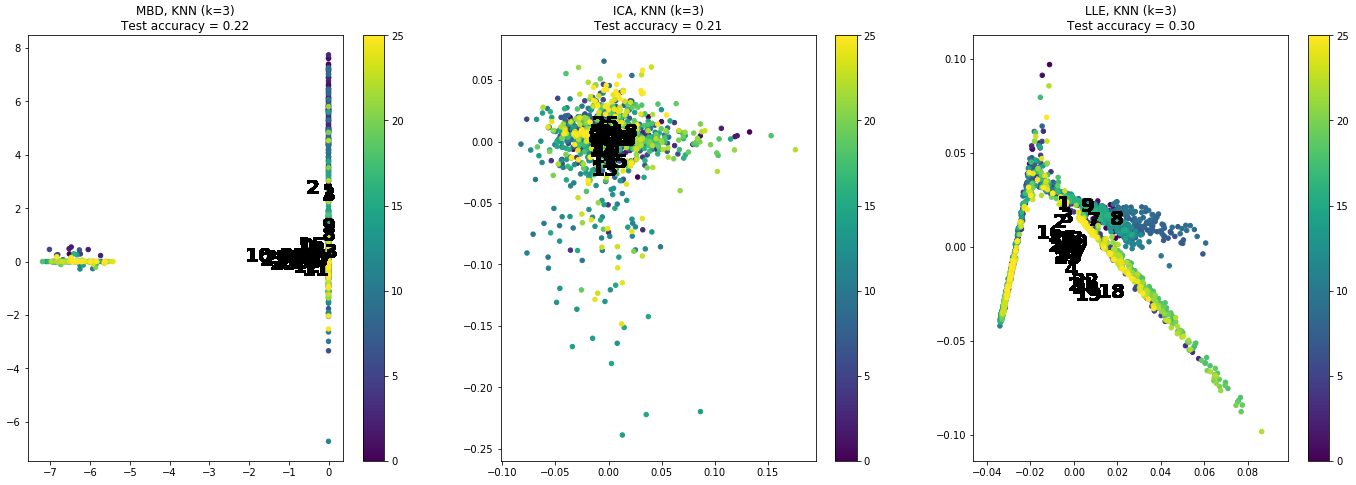
\includegraphics[width=.7\linewidth]{clustering_smg_d.png}}
\end{center}
\caption{Test of diferent methodos of dimensionality reduction for the use in the classificatory algorithm. The methods were tested with a \ac{KNN} with k =3.}
\label{fig_dim_reduction}
\end{figure}

%\begin{figure}[h]
%	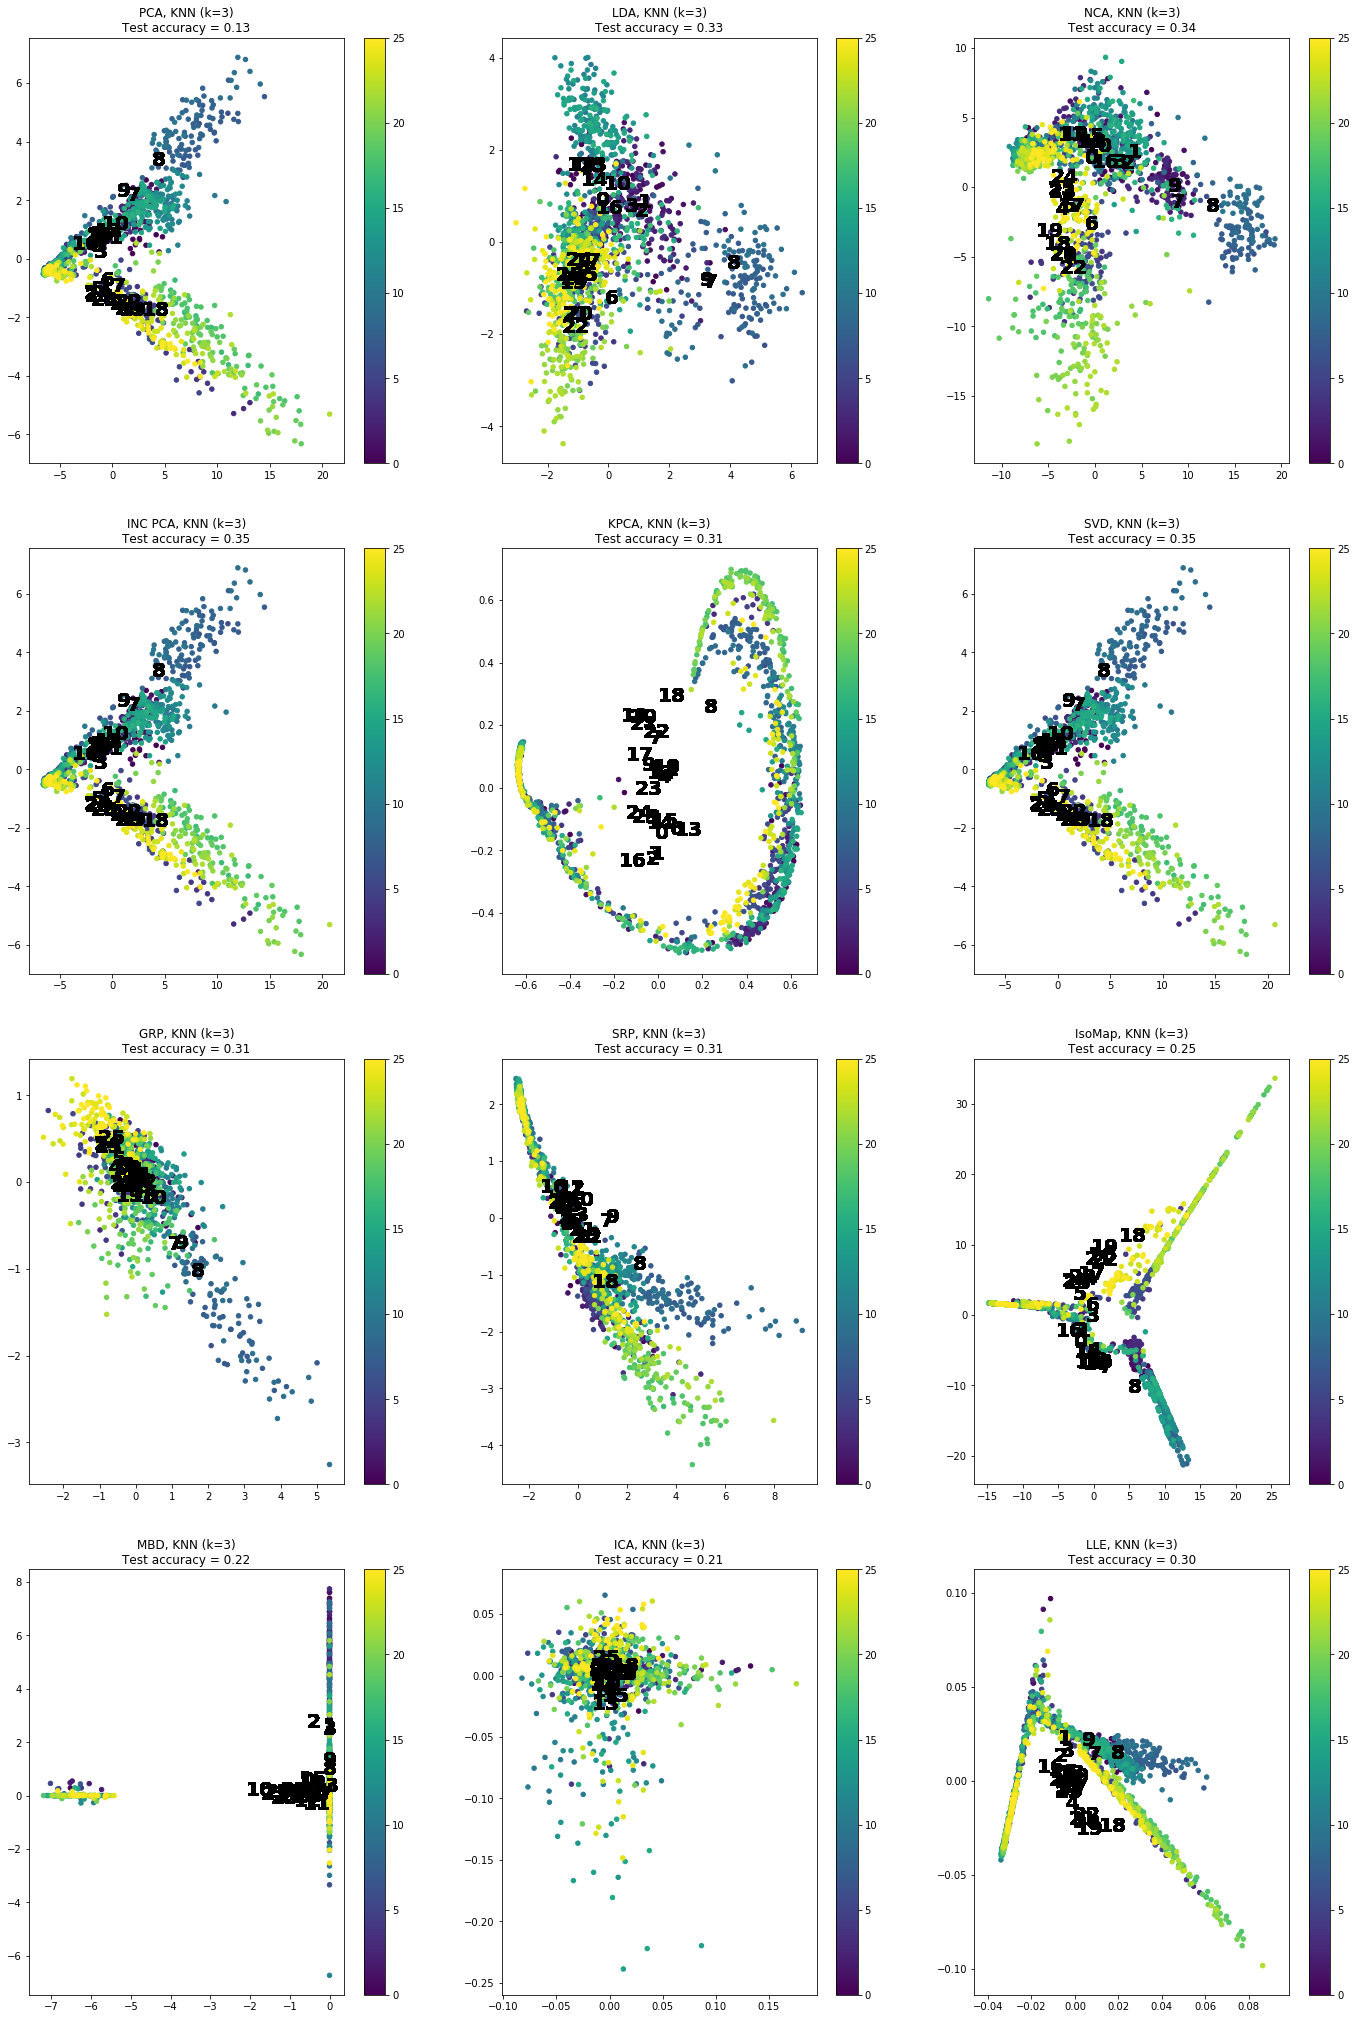
\includegraphics[scale=0.25]{clustering_smg.png}
%	\caption{Test of diferent methodos of dimensionality reduction for the use in the classificatory algorithm. The methods were tested with a KNN with k =3.} \label{fig_dim_reduction}
%\end{figure}

\subsection{Signal Information}

To extract the maximum information of the signal the processes were divided into two steps:

\begin{enumerate}
	\item Signal Clustering: Agglomerative Hierarchical Clustering (\ac{HCA}) clusterized the signal into three groups according to the similarity of the features. The HAC algorithm recursively merges the pair of clusters that minimally increases a given linkage distance~\cite{mainreferences}{Strbac2017,Gloumakov2019};
	\item Comparison with possible movements: after the creation of the cluster, the algorithm compares movements classes with the possible movements for a given position, and the classes are extracted through a process called Decision Tree or State Machine~\cite{mainreferences}{Delisle-Rodriguez2017}.
\end{enumerate}

\subsection{Classifier Algorithm}
A simple multi-layer perceptron (\ac{MLP}), with three layers, was used to classify the signal. The first layer was composed of 25 neurons, the middle layer by 52 neurons and the last by 26 neurons. In the first two layers, the linear rectifier was used as activation function. The last layer had a softmax function helping in the classification process. A dropout function (20\%), placed between the \ac{MLP} layers, reduce the chance of over-fitting.The \ac{MLP} was chosen because of its inherent capacity of simultaneous classification~\cite{mainreferences}{shannon1949mathematical}.

\begin{figure}[h]
    \begin{center}
	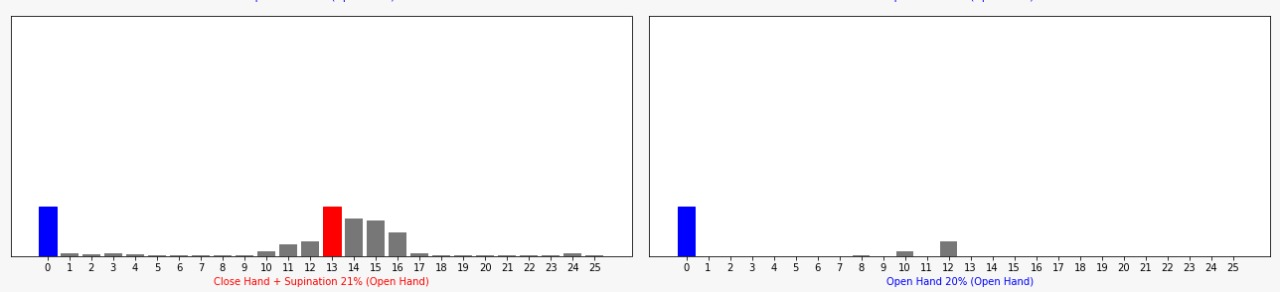
\includegraphics[width=.8\linewidth]{output.png}
	\end{center}
	\caption{Output of the values of the \ac{MLP} neurons of the last layer. The blue color mean the right classification and the red the wrong classification. The left figure is the output of the \ac{MLP} and the right figure is the result with the possible classes only.} \label{final_classification}
\end{figure}

\section{Results}

A recent study~\cite{mainreferences}{RadhikaMenonStudentMemberIEEEGaetanoDiCaterinaHebaLakanyMemberIEEELykourgosPetropoulakisBernardA.ConwayJohnJ.SoraghanSeniorMember} shows the impact of the temporal window size on the EMG signal classification error. According to this study, with very small windows, (on average less than 200 ms), the classification error increases as the total information in the window decreases. This feature makes real-time processing very difficult, since it requires small temporal windows. Moreover, in 2011 Peerdeman~\cite{mainreferences}{Peerdeman2011} found that the processing window needs to have less than 300 ms, or the delay becomes unacceptable to the user.

The proposals studied in this article aim to reduce this limit from 200 to 300 milliseconds by creating mechanisms that allow for using smaller windows. Through these smalltime windows, it is possible to perform real-time processing.

Because of the small size (10ms) of the window, the MLP did not achieve a good signal classification, but the selection of which neurons are active for the classification, significantly increased the accuracy. Figure 2 shows the difference in the classification using only the possible classes.

For the clustering algorithm, three data clusters were created and evaluated using a \ac{KNN} (k = 3). This \ac{KNN} achieved 97\% accuracy by classifying the groups created, as seen in figure \ref{fig_sMEG_Clustering}.

\begin{figure}[h]
	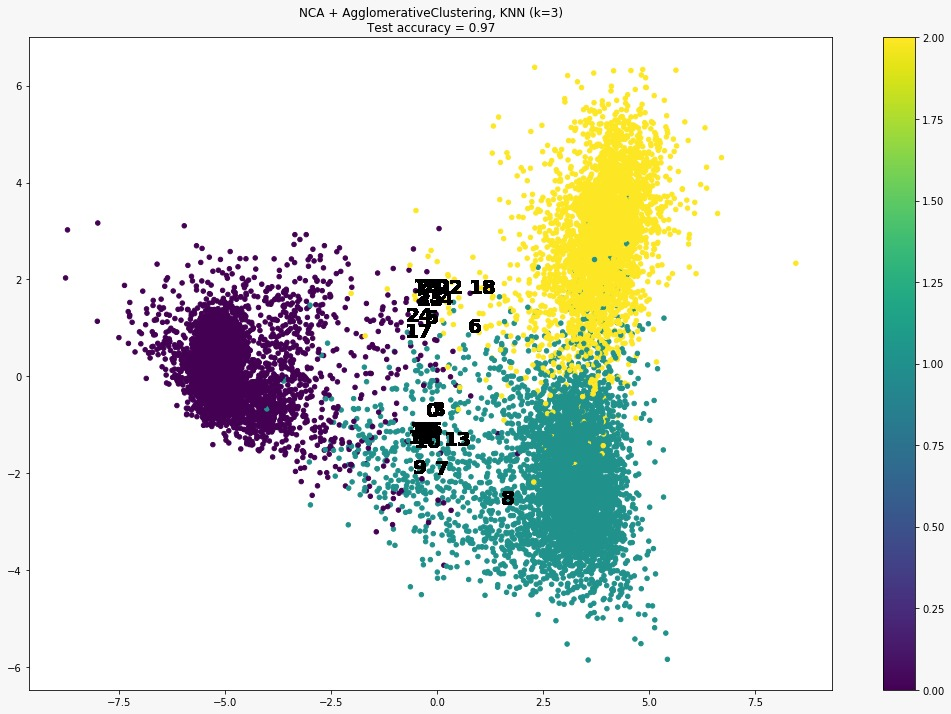
\includegraphics[width=\linewidth]{sMEG_Clustering.png}
	\caption{\ac{sMEG} Clustering the classes by the similarity in the features extracted. After the extraction of twenty-five dimensions, the two more representative dimensions among them were used to generate the plot. A \ac{KNN} was used to validate the cluster.} \label{fig_sMEG_Clustering}
\end{figure}

Table \ref{acc_std} shows the accuracy and standard deviation of \ac{MLP} used in this article. The left side shows the results for the full \ac{MLP}, and the right colulmn shows the, the results after the application of the pipeline shown in figure \ref{fig_class_fluxo}.

\begin{table}[h]
	\caption{Accuracy and Standard Deviation Comparison}
	\label{acc_std}
	\begin{center}
		\begin{tabular}{lll}
        \hline
                & Ful \ac{MLP} Output & \ac{MLP} with Selectd Neurouns \\ \hline
            Acc & 0.382          & 0.913                     \\
            Std & 0.013          & 0.011                     \\ \bottomrule
        \end{tabular}
	\end{center}
\end{table}

Although the standard deviation remained relatively unchanged, the improvement in accuracy was immense. This achievement can be reached by excluding very close classes, such as closing and flexing the hand or opening and flexing the hand, where misclassifications generally occur.

\section{Conclusion}

In this thesis, two methods were used to obtain a priori information and thus reduce signal entropy before classification. New methods can bring even more significant improvement to the system. By providing a priori information for signal classification interactively, the number of possible classes for signal classification dramatically decreases. Creating less complex validation steps also increased accuracy while allowing window size reduction. We believe that the techniques presented here only scratch the surface of the applications where information entropy can and should be used.

The main idea of this study was to create a network that is simple and, through a small number of bits, can generalize the data better than a more complex network. Therefore, it is imperative to provide tools that simplify or provide data information. Besides, a simple neural network will have faster processing time and use less energy, being cheaper to train and more efficient to apply. Thus, providing tools that simplify or provide data information is critical. Furthermore, more studies to account for the trade-off between the number of steps and the processing time of the pipeline is needed.

\chapter{Conclusion}\label{chap:Conclusao}

This study was done with the intention of raising a greater amount of information about the \ac{EMG} signal. This survey serves to build a better definition of the problem. Knowing how the signal behaves it is possible to create simpler and more efficient solution. For this purpose, a processing protocol of feature extraction, clustering and classification of the myo-electric signal were followed.

As a good prosthesis experience needs quick responses, real-time processing is critical. The number of features and their choice was such as to guarantee faster signal processing. Four characteristics in the frequency domain were selected: 
\begin{itemize}
    \item Spectral Moment;
    \item Waveform Length (cumulative changes in the length);
    \item Mean;
    \item Median;
\end{itemize}

One of the difficulties in classifying the signal was knowing exactly where the movement started. This happens because of the stochastic characteristics of the signal, when motor units start to be recruited, the signal of rest and movement are confused. To differentiate these two states, a variational self-hiding was used. Due to its intrinsic characteristics, it is specialized in separating classes (movement and rest) in its latent layer. With a simple perceptron it was possible to ascertain the change in the user's states and activate the prosthesis movement classifier.

The last part of this study was the development of a classifier. For this, the concept of information entropy was used. The first part of the classifier was the construction of a state machine that maps the possible combinations of movement given an initial position of the prosthesis. Another step was the use of clusters to catalog nearby movements, the intersection of these two steps generates a list of possible movements. Because of the extremely small time window, without using these two steps, classification would be impossible.

Since the myo-electric prostheses were developed, the number of users who reject it has remained constant~\cite{mainreferences}{Brook1985}, Which shows that there has been no significant advance in the area. The reduction of the time window for the classification of the myo-electric signal will allow the control of the prosthesis to be performed in a more fluid way by the user, increasing his comfort when using it.

Another very important factor generated by the decrease in the time window is the decrease in the complexity of the evaluation, which results in energy savings during the classification process, which, in turn, would increase the time of using the prosthesis, reducing the amount of time of refills that the user would need to do. In addition, the processing developed in this study can be used for the classification of other natural signals which, as they are diluted (too much information for little information), are difficult to classify.

The collection of \ac{EMG} signal data can be stressful for the patient, so it is very difficult to get large databases of biological signals. Because of this, this study was done using only one database, provided along with the BioPatRec platform. In addition, the database used has few repetitions of movement, which makes training with machine learning algorithms difficult. In total, this base has only 17 patients and 3 repetitions of each movement, which made it impossible to use some training techniques.

With a sufficiently large database and, once a redundant classifier has been created, as in the case of the study, the various steps of the cassification can be used as a code and, with a larger neural network and the values of the classification windows can be predicted using techniques such as \ac{LSTM}.

One of the main future works would be the implementation of the system and tests with patients with live acquisition of the \ac{sEMG}. The corelations between the time windows can also be studied in order to have a better designed classifier. New methods of reducing entropy before the classifier mustbe tested since tools that simplify or provide data information is critical.

Despite the few samples of the data set used, the methodology created in this thesis proved to be efficient for the classification of the \ac{sEMG} signal. However, further studies must be carried out to find new ways to decrease the entropy of the signal before its final classification.

\renewcommand\bibname{\Large\scshape References}
\addcontentsline{toc}{chapter}{\bf References}
\bibliography{mainreferences}{referencias}{References}

\end{document} 
%---}}}
